\def\GraphicsFolder{chapters/antiferromagnetic-instability/pictures}
\chapter{Antiferromagnetic instability}\label{chap:mft-af-instability}

This chapter is devoted to an in-depth discussion of the antiferromagnetic (AF) long-range ordering in the EHM by the means of MFT. In the context of the $2$D HM, discussed in App.~\ref{appendix:mean-field-hubbard}, AF ordering establishes as an unconventional metallic phase which is only stable at half-filling (as is discussed in Sec.~\ref{appsubsec:af-instability}). The situation for the EHM is similar: the present analysis is carried out based on the argument that, given the symmetry structure of the non-local NN interaction, the fundamental features of the commensurate AF phase of the HM are effectively preserved, while the parameters are redefined by the interaction itself. The two most relevant effects we discuss in this chapter are the gap ``complexification'' and the bands renormalization and resymmetrization (both in Sec.~\ref{sec:af-fock-bands-renormalization}), the latter being a general feature of the EHM common to all phases preserving (or, at most, weakening without destroying) translational invariance, discussed previously in Sec.~\ref{sec:normal-fock-bands-renormalization}.

\section{The AF phase and its symmetries}\label{sec:af-phase-theory}

%When discussing the AF phase on the EHM on square lattice, we must specify the type of antiferromagnetism we are dealing with. SDW antiferromagnets on a square lattice can emerge in a variety of ways, the simplest one -- described in this text -- being the so-called ``commensurate''. By this we mean essentially a kind of long range spin density ordering varying on the length scale of two lattice sites. This type of AF structure is particularly interesting on a square lattice because the phase transition is simply described in reciprocal space by the order parameter 
%\[
%	\hat \psi_{\mathbf{k}\sigma} \equiv \hat c_{\mathbf{k}+\bm{\pi}\sigma}^\dagger \hat c_{\mathbf{k}\sigma}
%\]
%going from a null EV in the normal phase to a non-zero value. This phenomenon occurs at the so called ``AF vector''
%\[
%	\bm{\pi} \equiv (\pi,\pi)
%\]
%Large portions of a square lattice Fermi surface (FS) can turn out to be connected precisely by an AF vector: this implies that, if the hamiltonian makes available a scattering channel at this wavevector, electrons can jump from one side to the other, making said EV non-zero.
%
%In principle, the AF phase is physically established by breaking the $\mathrm{SU}(2)$ spin rotation symmetry down to the $\mathrm{U}^z(1)$ projected spin rotation symmetry; however, it is to be noted that -- even if the concept of SSB is well defined only for the $\mathrm{SU}(2) \to \mathrm{U}^z(1)$ symmetry reduction -- the hamiltonian in thermodynamic limit remains $\mathbb{Z}_2$ invariant with respect to spin inversion, $\sigma \leftrightarrow \overline{\sigma}$. Identical considerations as in Sec.~\ref{sec:normal-phase-theory} hold This: all physical quantities are spin-independent. As for the normal phase, we will use this considerations at the end of the calculations. 

The AF phase is not uniquely defined; actually, there exists a variety of ways to establish a SDW phase in a spin-balanced square lattice, which means a system where both spin sectors are equally populated, but differently displaced. {\color{tabred}[ToDo: graphics of various SDW structures]}

The AF phase hereby presented is a symmetry reduction of the normal phase, and is described by simultaneous spin rotational symmetry reduction and translational symmetry halving:
\[
\begin{aligned}
	\mathrm{SU}(2) &\SSB \mathrm{U}^z(1) \\
	\mathrm{T}_1^{(x)} \otimes \mathrm{T}_1^{(y)} &\SSB \mathrm{T}_2^{(x)} \otimes \mathrm{T}_2^{(y)}
\end{aligned}
\]
We describe a SDW whose period is of two sites. As done for the normal phase, we allow theoretically
\[
	\mathrm{C}_4 \SSB \mathrm{C}_2
\]
in order to capture the same anisotropy effects seen in Sec.~\ref{subsec:normal-fock-analytic}. 

Recall Tabs.~\ref{tab:U-wick-terms-phases} and \ref{tab:V-wick-terms-phases}, collecting the RWCs for the AF phase,
\[
\begin{aligned}
	&\hat H_U 
	&&\text{Hartree contraction} \\
	&\hat H_V \text{ (o.s. sector)}
	&&\text{Hartree contraction} \\
	&\hat H_V \text{ (s.s. sector)}
	&&\text{Hartree and Fock contractions} \\
\end{aligned}	
\]
We anticipate the role of all RWCs in Tab.~\ref{tab:af-RWCs}.

\begin{table}[t]
	\centering
	\begin{tabular}{c c c l}
		\textbf{Operator} & \textbf{Sector} & \textbf{RWCs} & \textbf{Net effect} \\
		\midrule
		$\hat H_U$ && Hartree & $\mu$ shift by $-nU$ \\
		\midrule
		\multirow{4}{*}{$\hat H_V$} & o.s. & Hartree & $\mu$ shift by $nzV$ \\[0.5em]
		& \multirow{3}{*}{s.s.} & Hartree & $\mu$ shift by $nzV$\\
		&& \multirow{2}{*}{Fock} & Bands renormalization and resymmetrization,\\
		& & & gap complexification \\
		\midrule
	\end{tabular}
	\caption{Relevant Wick's contractions and net effect in the AF phase. Note the similarity with Tab.~\ref{tab:normal-RWCs}.}
	\label{tab:af-RWCs}
\end{table}

\subsection{Antiferromagnetism in the HM}\label{subsec:af-hm}

In this short section we recall the principal features of the AF phase established in the conventional HM, discussed in Sec.~\ref{appsec:antiferromagnetic-phase}. Before starting, let us define as in Eqns.~\eqref{appeq:af-hm-psi-def} and \eqref{appeq:af-hm-n-def} the AF and density fluctuations operators,
\begin{align}
	\hat n_{\mathbf{k}\sigma} &\equiv \hat c_{\mathbf{k}\sigma}^\dagger \hat c_{\mathbf{k}\sigma} \label{eq:af-ehm-n-def} \\
	\hat \psi_{\mathbf{k}\sigma} &\equiv \hat c_{\mathbf{k}+\bm{\pi}\sigma}^\dagger \hat c_{\mathbf{k}\sigma} \label{eq:af-ehm-psi-def}
\end{align}
which represent the two essential fermionic quadratic operators of the analytic MFT derivation. It is very useful to also note the following properties. Given the $\gamma$-wave form factors of Tab.~\ref{tab:x-wave-reciprocal-factors}, evidently both the following equations hold
\[
\begin{aligned}
	\hat \psi_{\mathbf{k}+\bm{\pi}\sigma}^\dagger &= \hat \psi_{\mathbf{k}\sigma} \\
	\varphi_{\mathbf{k}+\bm{\pi}}^{(\gamma)} &= -\varphi_\mathbf{k}^{(\gamma)}
\end{aligned}
\]
which imply the handy property
\begin{equation}\label{eq:af-ehm-vphi-psi-property}
	\varphi_{\mathbf{k}+\bm{\pi}}^{(\gamma)} \psi_{\mathbf{k}+\bm{\pi}\sigma}^\dagger = - \varphi_\mathbf{k}^{(\gamma)} \psi_{\mathbf{k}\sigma}
\end{equation}

Within the pure HM, the AF phase is specified by the Ansatz \eqref{appeq:af-mean-field-ansatz},
\begin{equation}\label{eq:af-mean-field-ansatz}
	\langle \hat n_{\mathbf{r}\sigma} \rangle = n - (-1)^{x+y+\delta_{\sigma=\uparrow}} m
\end{equation}
which is explicitly breaking translational invariance in each spin sector, while preserving $\mathrm{U}^z(1)$ and $\mathrm{U}^c(1)$ symmetries. As reported in Tab.~\ref{tab:U-wick-terms-phases}, the only RWC comes in Hartree channel, since the local two-body interaction couples operators at opposite spin index. The hamiltonian $\hat H$ is reduced thereby to the form of Eq.~\eqref{appeq:af-hm-mft-h}
\begin{multline*}
	\hat H_t + \hat H_U \stackrel{\mathrm{MFT}}{\simeq} -t \sum_{\langle \mathbf{r}\mathbf{r}' \rangle} \sum_\sigma 
	\left[
		\hat c_{\mathbf{r}\sigma}^\dagger \hat c_{\mathbf{r}'\sigma} + \hc
	\right]
	+ nU \sum_\mathbf{r} \left[
		\hat n_{\mathbf{r}\uparrow} + \hat n_{\mathbf{r}\downarrow}
	\right] \\
	- mU \sum_\mathbf{r} (-1)^{x+y} \left[
		\hat n_{\mathbf{r}\uparrow} - \hat n_{\mathbf{r}\downarrow}
	\right] - E_{\mathrm{H}/U}^{(\mathrm{AF})}
\end{multline*}
with $E_{\mathrm{H}/U}^{(\mathrm{AF})}$ the contraction energy resulting from double counting terms, given explicitly in Eq.~\eqref{appeq:af-hm-hartree-U-Ec},
\[
	E_{\mathrm{H}/U}^{(\mathrm{AF})} = L_x L_y \times U \left(
		n^2 - m^2
	\right)
\]
In reciprocal space, the hamiltonian decomposes as in Eq.~\eqref{af-hm-bogoliubov-h},
\[
	\hat H_t + \hat H_U \stackrel{\mathrm{MFT}}{\simeq} \sum_{\mathbf{k} \in \mathrm{MBZ}} \sum_\sigma \hat \Psi_{\mathbf{k}\sigma}^\dagger h_{\mathbf{k}\sigma} \hat \Psi_{\mathbf{k}\sigma} + nU \times \hat N - E_{\mathrm{H}/U}^{(\mathrm{AF})}
	\qq{being}
	h_{\mathbf{k}\sigma} \equiv \begin{bmatrix}
		\epsilon_{\mathbf{k}\sigma} & -\Delta_{\mathbf{k}\sigma}^* \\
		-\Delta_{\mathbf{k}\sigma} & - \epsilon_{\mathbf{k}\sigma}
	\end{bmatrix}
\]
and $\Delta_{\mathbf{k}\sigma} = (-1)^{\delta_{\sigma=\downarrow}}mU$. Nambu spinorial formulation is used,
\[
\hat \Psi_{\mathbf{k}\sigma} \equiv \begin{bmatrix}
	\hat c_{\mathbf{k}\sigma} \\
	\hat c_{\mathbf{k}+\bm{\pi}\sigma} 
\end{bmatrix}
\]
and the free electrons energy is simply the tight binding energy of Eq.~\eqref{eq:bare-bands} written with an explicit spin index,
\[
	\epsilon_{\mathbf{k}\sigma} = -2t \left(
		\cos k_x + \cos k_y
	\right)
\]
which is spin-invariant. The MFT description of the model reduces to a gas of free ``$\gamma$-fermions'', described by the Nambu spinor of Eq.~\eqref{appeq:af-hm-Gamma-WPsi},
\[
	\hat\Gamma_{\mathbf{k}\sigma} = W_{\mathbf{k}\sigma} \hat \Psi_{\mathbf{k}\sigma} = \begin{bmatrix}
		\hat \gamma_{\mathbf{k}\sigma}^{(+)} \\ \hat \gamma_{\mathbf{k}\sigma}^{(-)}
	\end{bmatrix}
\]
where
\[
	W_{\mathbf{k}\sigma} = \begin{bmatrix}
		\cos \theta_{\mathbf{k}\sigma} & - \sin \theta_{\mathbf{k}\sigma} \\
		\sin \theta_{\mathbf{k}\sigma} & \cos \theta_{\mathbf{k}\sigma}
	\end{bmatrix}
	\qq{and}
	\sin 2\theta_{\mathbf{k}\sigma} \equiv \frac{\Delta_{\mathbf{k}\sigma}}{E_{\mathbf{k}\sigma}}
\]
These fermions populate the two bands $\pm E_{\mathbf{k}\sigma} = \sqrt{\epsilon_{\mathbf{k}\sigma}^2 + \abs{\Delta_{\mathbf{k}\sigma}}^2}$. The entire system is mapped onto an ensemble of pseudo-spins, each subject to a pseudo-field, as in Fig.~\ref{fig:pseudo-magnetic-field}. To diagonalize the system essentially means to anti-align each pseudo-spin with the $z$ axis. Each pseudospin component expectation value (EV) is described by a simple equation and has a precise meaning, listed in Tab.~\ref{tab:af-pseudospin-map}.

\begin{table}
	\centering
	\begin{tabular}{c c c}
		\textbf{EV} & \textbf{Meaning} & \textbf{Equation} \\
		\midrule
		$\ev{\hat s_{\mathbf{k}\sigma}^x}$ & $\ev{
			\hat \psi_{\mathbf{k}\sigma}
			+ \hat \psi_{\mathbf{k}\sigma}^\dagger
		}$ & \eqref{appeq:af-hm-sx} \\[0.7em]
		$\ev{\hat s_{\mathbf{k}\sigma}^y}$ & $i \ev{
			\hat \psi_{\mathbf{k}\sigma}
			- \hat \psi_{\mathbf{k}\sigma}^\dagger
		}$ & \eqref{appeq:af-hm-sy} \\[0.7em]
		$\ev{\hat s_{\mathbf{k}\sigma}^z}$ & $\ev{
			\hat n_{\mathbf{k}\sigma}
			+ \hat n_{\mathbf{k}+\bm{\pi}\sigma}
		}$ & \eqref{appeq:af-hm-sz} \\
		\midrule
	\end{tabular}
	\caption{List of the various expectation values (EVs) of each pseudospin component, their meaning in terms of fermionic operators and the reference equations from the pure HM.}
	\label{tab:af-pseudospin-map}
\end{table}

\subsection{Extension to the EHM}\label{subsec:af-ehm}

Consider now the non-local interaction $\hat H_V$. Being the RWCs the same as for the normal phase, the discussion is essentially the same of Chap.~\ref{chap:normal-phase}, with the only relevant difference being the Ansatz we use in Eq.~\eqref{eq:normal-density-ansatz}, substituted by the commensurate oscillatory Ansatz of Eq.~\eqref{eq:af-mean-field-ansatz}. {\color{tabred} By itself, even if it may seem the contrary, the Ansatz does not imply $\mathrm{C}_4$ symmetry preservation. It is possible to reduce point group symmetry having still a rotation-symmetric magnetization, as well as it was possible to do in the normal phase with keeping a uniform density.} As for the normal phase, by design the MFT solution to the model for the given phase is described by a redefinition of the various physical quantities and mathematical objects,
\[
	\epsilon_{\mathbf{k}\sigma} \to \tilde{\epsilon}_{\mathbf{k}\sigma}
	\qquad
	E_{\mathbf{k}\sigma} \to \tilde{E}_{\mathbf{k}\sigma}
	\qquad
	\Delta_{\mathbf{k}\sigma} \to \tilde{\Delta}_{\mathbf{k}\sigma}
	\qquad
	\mu \to \tilde{\mu}
\]
The band energies renormalization is simply
\[
	\tilde{E}_{\mathbf{k}\sigma} \equiv \sqrt{\tilde{\epsilon}_{\mathbf{k}\sigma}^2 + |\tilde{\Delta}_{\mathbf{k}\sigma}|^2}
\]
and the following relations hold (the \textit{tilde} sign indicates the renormalized quantity):
\begin{align}
	\langle \hat \Psi_{\mathbf{k}\sigma}^\dagger \tau^x \hat \Psi_{\mathbf{k}\sigma} \rangle &= -\sin 2\tilde{\theta}_{\mathbf{k}\sigma} \cos 2\tilde{\zeta}_{\mathbf{k}\sigma} \langle \hat \Gamma_{\mathbf{k}\sigma}^\dagger \tau^z \hat \Gamma_{\mathbf{k}\sigma} \rangle \label{eq:af-x-expectation-non-local}\\
	\langle \hat \Psi_{\mathbf{k}\sigma}^\dagger \tau^y \hat \Psi_{\mathbf{k}\sigma} \rangle &= -\sin 2\tilde{\theta}_{\mathbf{k}\sigma} \sin 2\tilde{\zeta}_{\mathbf{k}\sigma} \langle \hat \Gamma_{\mathbf{k}\sigma}^\dagger \tau^z \hat \Gamma_{\mathbf{k}\sigma} \rangle \label{eq:af-y-expectation-non-local}\\
	\langle \hat \Psi_{\mathbf{k}\sigma}^\dagger \tau^z \hat \Psi_{\mathbf{k}\sigma} \rangle &= \cos 2\tilde{\theta}_{\mathbf{k}\sigma} \langle \hat \Gamma_{\mathbf{k}\sigma}^\dagger \tau^z \hat \Gamma_{\mathbf{k}\sigma} \rangle \label{eq:af-z-expectation-non-local}
\end{align}
equivalent to the ones for the pure HM, Eqns.~\eqref{appeq:af-hm-sx}, \eqref{appeq:af-hm-sy} and \eqref{appeq:af-hm-sz}. Moving to the the tilted frame, the $z$ component of the pseudospin is just a thermal superposition of the ``up'' and ``down'' states
\begin{equation}\label{eq:af-rot-z-expectation}
	\langle \hat \Gamma_{\mathbf{k}\sigma}^\dagger \tau^z \hat \Gamma_{\mathbf{k}\sigma} \rangle =
	f\left(
		\tilde{E}_{\mathbf{k}\sigma};\beta,\tilde{\mu}
	\right) - f\left(
		-\tilde{E}_{\mathbf{k}\sigma};\beta,\tilde{\mu}
	\right)
\end{equation}
Let us define the (renormalized) thermal factors as in Eq.~\eqref{appeq:af-thermal-factors-def},
\begin{equation}\label{eq:af-ren-thermal-factors-def}
	\tilde{\mathrm{Th}}_{\mathbf{k}\sigma}^{(\pm)}[\beta,\tilde{\mu}] \equiv 
	f\left(
		-\tilde{E}_{\mathbf{k}\sigma};\beta,\tilde{\mu}
		\right) \pm f\left(
		\tilde{E}_{\mathbf{k}\sigma};\beta,\tilde{\mu}
	\right)
\end{equation}
The angles satisfy: \begin{equation}\label{eq:af-bogoliubov-angle-relations}
	\sin 2\tilde{\xi}_{\mathbf{k}\sigma} = \frac{\Re\{\tilde{\Delta}_{\mathbf{k}\sigma}\}}{|\tilde{\Delta}_{\mathbf{k}\sigma}|}
	\quad
	\cos 2\tilde{\xi}_{\mathbf{k}\sigma} = \frac{\Im\{\tilde{\Delta}_{\mathbf{k}\sigma}\}}{|\tilde{\Delta}_{\mathbf{k}\sigma}|}
	\quad
	\sin 2\tilde{\theta}_{\mathbf{k}\sigma} = \frac{|\tilde{\Delta}_{\mathbf{k}\sigma}|}{\tilde{E}_{\mathbf{k}\sigma}}
	\quad
	\cos 2\tilde{\theta}_{\mathbf{k}\sigma} = \frac{\tilde{\epsilon}_{\mathbf{k}\sigma}}{\tilde{E}_{\mathbf{k}\sigma}}
\end{equation}
The physical behaviour is the same as for the pure HM. In terms of MFT discussion, the AF phase is similar enough to the normal phase of Chap.~\ref{chap:normal-phase}: the RWCs are the same of Sec.~\ref{sec:normal-phase-theory}, listed in Tabs.~\ref{tab:U-wick-terms-phases} and \ref{tab:V-wick-terms-phases}. All three Hartree contractions, responsible in the normal phase for the chemical potential shift, and the s.s. Fock contraction, that originated the hopping renormalization. Let us start by the Hartree terms: due to the ``staggered'' nature of the commensurate AF phase, their role is here more complex. Then we will move to the Fock term, discussing the MFT approximations effect on bands. Next sections are basically an extension of the calculations of Chap.~\ref{chap:normal-phase}.

\begin{figure}
	\centering
	\input{\GraphicsFolder/pseudo-magnetic-field}
	\caption{Sketch of the diagonalization of the pseudo-spin problem. The dashed line represents the diagonalization given by the $z$-axis alignment with the field direction. In the top-right side of the picture are listed the expectation values of the original Nambu spinor. For simplicity everywhere the index $\sigma=\uparrow$ has been omitted.}
	\label{fig:pseudo-magnetic-field}
\end{figure}

\section{Non-local Hartree effects: chemical potential renormalization}\label{subsec:af-hartree-mu}

As in Eq.~\eqref{eq:normal-V-wick-decomposition}, the same-spin and opposite-spin non-local Hartree terms are
\begin{multline*}
	\hat H_V \simeq
	\overbrace{
		-V \sum_{\ev{ij}} \sum_\sigma \left[
			\langle
			\hat n_{i\sigma}
			\rangle \hat n_{j\sigma} + \hat n_{i\sigma} \langle
			\hat n_{j\sigma}
			\rangle - \langle
			\hat n_{i\sigma}
			\rangle \langle
			\hat n_{j\sigma}
			\rangle
		\right]
	}^{\mathrm{s.s.}} \\
	\underbrace{
		-V \sum_{\ev{ij}} \sum_\sigma \left[
			\langle
			\hat n_{i\sigma}
			\rangle \hat n_{j\overline{\sigma}} + \hat n_{i\sigma} \langle
			\hat n_{j\overline{\sigma}}
			\rangle
			- \langle
			\hat n_{i\sigma}
			\rangle \langle
			\hat n_{j\overline{\sigma}}
			\rangle
		\right]
	}_{\mathrm{o.s.}} \, +\,
	(\text{all the rest})
\end{multline*}
Let $i \to \mathbf{r} = (x,y)$ and $j \to \mathbf{r}' = (x',y')$. We use Eq.~\eqref{eq:af-mean-field-ansatz}, which describes an oscillatory density for each spin sector. This Ansatz is composed of two parts: the offset $n$, and the oscillatory part $m$. The algebraic derivation relative to the $n$ part is, of course, the same as for the normal phase. We now treat separately the ``operatorial'' part of the braced terms of Eq.~\eqref{eq:normal-V-wick-decomposition},
\begin{equation}\label{eq:af-V-wick-decomposition-operatorial}
	-V \sum_{\ev{\mathbf{r}\mathbf{r}'}} \sum_\sigma \left[
		\langle
		\hat n_{\mathbf{r}\sigma}
		\rangle \hat n_{\mathbf{r}'\sigma} + \hat n_{\mathbf{r}\sigma} \langle
		\hat n_{\mathbf{r}'\sigma}
		\rangle
		\right] -V \sum_{\ev{\mathbf{r}\mathbf{r}'}} \sum_\sigma \left[
		\langle
		\hat n_{\mathbf{r}\sigma}
		\rangle \hat n_{\mathbf{r}'\overline{\sigma}} + \hat n_{\mathbf{r}\sigma} \langle
		\hat n_{\mathbf{r}'\overline{\sigma}}
		\rangle
	\right]
\end{equation}
as well as the its scalar counterpart
\begin{equation}\label{eq:af-V-wick-decomposition-double-counting}
	V \sum_{\ev{\mathbf{r}\mathbf{r}'}} \sum_\sigma
	\langle \hat n_{\mathbf{r}\sigma} \rangle \langle \hat n_{\mathbf{r}'\sigma} \rangle + V \sum_{\ev{\mathbf{r}\mathbf{r}'}} \sum_\sigma
	\langle \hat n_{\mathbf{r}\sigma} \rangle \langle \hat n_{\mathbf{r}'\overline{\sigma}} \rangle
\end{equation}
which accounts for the energy shift to be accounted when performing Wick's contractions.

\subsection{Hartree channel in the AF phase: analytic derivation}\label{subsec:af-hartree-analytic}

Let us start from the operator of Expr.~\eqref{eq:af-V-wick-decomposition-operatorial}. By inserting the Ansatz of Eq.~\eqref{appeq:af-mean-field-ansatz}, we get
\begin{multline*}
	\overbrace{
		-nV \sum_{\ev{\mathbf{r}\mathbf{r}'}} \sum_\sigma \left[
		\hat n_{\mathbf{r}'\sigma} + \hat n_{\mathbf{r}\sigma}
		\right] + mV \sum_{\ev{\mathbf{r}\mathbf{r}'}} \sum_\sigma (-1)^{\delta_{\sigma=\uparrow}} \left[
		(-1)^{x+y} \hat n_{\mathbf{r}'\sigma} + (-1)^{x'+y'} \hat n_{\mathbf{r}\sigma}
		\right]
	}^{\mathrm{s.s.}} \\
	\underbrace{
		-nV \sum_{\ev{\mathbf{r}\mathbf{r}'}} \sum_\sigma \left[
		\hat n_{\mathbf{r}'\overline{\sigma}} + \hat n_{\mathbf{r}\sigma}
		\right] + mV \sum_{\ev{\mathbf{r}\mathbf{r}'}} \sum_\sigma \left[
		(-1)^{x+y+\delta_{\sigma=\uparrow}} \hat n_{\mathbf{r}'\overline{\sigma}} + (-1)^{x'+y'+\delta_{\overline{\sigma}=\uparrow}} \hat n_{\mathbf{r}\sigma}
		\right]
	}_{\mathrm{o.s.}}
\end{multline*}
For a square lattice, if $\mathbf{r} = (x,y)$ and $\mathbf{r}' = (x',y')$ are NNs, evidently
\[
\begin{aligned}
	(-1)^{x'+y'} &= (-1)^{x+y+1} \\
	(-1)^{\delta_{\overline{\sigma}=\uparrow}} &= (-1)^{\delta_{\sigma=\uparrow}+1}
\end{aligned}
\]
We obtain
\begin{multline}
	\overbrace{
		-nV \sum_{\ev{\mathbf{r}\mathbf{r}'}} \sum_\sigma \left[
		\hat n_{\mathbf{r}\sigma} + \hat n_{\mathbf{r}'\sigma}
		\right]
	}^{\text{s.s. (density)}} - \overbrace{
		mV \sum_{\ev{\mathbf{r}\mathbf{r}'}} \sum_\sigma (-1)^{x+y+\delta_{\sigma=\uparrow}} \left[
		\hat n_{\mathbf{r}\sigma} - \hat n_{\mathbf{r}'\sigma}
		\right]
	}^{\text{s.s. (magnetization)}} \\
	\underbrace{
		-nV \sum_{\ev{\mathbf{r}\mathbf{r}'}} \sum_\sigma \left[
		\hat n_{\mathbf{r}\sigma} + \hat n_{\mathbf{r}'\overline{\sigma}}
		\right]
	}_{\text{o.s. (density)}} + \underbrace{
		mV \sum_{\ev{\mathbf{r}\mathbf{r}'}} \sum_\sigma (-1)^{x+y+\delta_{\sigma=\uparrow}} \left[
		\hat n_{\mathbf{r}\sigma} + \hat n_{\mathbf{r}'\overline{\sigma}}
		\right]
	}_{\text{o.s. (magnetization)}}
	\label{eq:af-ehm-hartree-int-1}
\end{multline}
In the above expressions the various contribution have been separated in ``density'' contributions and ``magnetization'' contributions. Let us deal with these separately.

\paragraph{Density terms.}

Consider the s.s. and o.s. (density) terms of Expr.~\eqref{eq:af-ehm-hartree-int-1},
\begin{equation}\label{eq:af-hartree-renormalization-density}
	-nV \sum_{\ev{\mathbf{r}\mathbf{r}'}} \sum_\sigma \left[
	\hat n_{\mathbf{r}\sigma} + \hat n_{\mathbf{r}'\sigma}
	\right] -nV \sum_{\ev{\mathbf{r}\mathbf{r}'}} \sum_\sigma \left[
	\hat n_{\mathbf{r}\sigma} + \hat n_{\mathbf{r}'\overline{\sigma}}
	\right]
\end{equation}
The discussion is identical to the one of Sec.~\ref{subsec:normal-hartree-analytic} for the normal phase, with the renormalization of $\mu$ being the same of Eq.~\eqref{eq:normal-mu-shift}.
\begin{equation}\label{eq:af-mu-shift}
	\tilde{\mu} \equiv \mu + n(2zV-U)
\end{equation}
Within this equation we are also already implicitly considering the $\mu$ shift effect due to $\hat H_U$., discussed both in Sec.~\ref{sec:normal-hartree-mu} and Sec.~\ref{appsubsec:af-hartree-channel}.

\paragraph{Magnetization terms.}

The $\mathrm{s.s.}$ and $\mathrm{o.s.}$ (magnetization) terms of Expr.~\eqref{eq:af-ehm-hartree-int-1} perfectly cancel out:
\[
	mV \sum_{\ev{\mathbf{r}\mathbf{r}'}} \sum_\sigma (-1)^{x+y+\delta_{\sigma=\uparrow}} \left[
		\left(
			\hat n_{\mathbf{r}\sigma} - \hat n_{\mathbf{r}'\sigma}
		\right) - \left(
			\hat n_{\mathbf{r}\sigma} + \hat n_{\mathbf{r}'\overline{\sigma}}
		\right)
	\right] = 0
\]
thus the only net effect of the Hartree RWCs affects $\mu$. This is somewhat to be expected: in the context of the HM, the gap function emerges in its purely $s$-wave structure from this precise computation on Hartree terms. However, the $\hat H_V$ non-local interaction cannot provide a pure $s$-wave potential component. Effects on the gap function are to be observed somewhere else.

%are to be reduced to a renormalization of the gap function. Explicitly,
%\begin{multline}
%	mV \sum_{\ev{\mathbf{r}\mathbf{r}'}} \sum_\sigma (-1)^{x+y+\delta_{\sigma=\uparrow}} \left[
%	\hat n_{\mathbf{r}\sigma} - \hat n_{\mathbf{r}'\sigma}
%	\right] + mV \sum_{\ev{\mathbf{r}\mathbf{r}'}} \sum_\sigma (-1)^{x+y+\delta_{\sigma=\uparrow}} \left[
%	\hat n_{\mathbf{r}\sigma} + \hat n_{\mathbf{r}'\overline{\sigma}}
%	\right] \\
%	= -2zmV \sum_\mathbf{r} (-1)^{x+y} \left[
%	\hat n_{\mathbf{r}\uparrow} - \hat n_{\mathbf{r}\downarrow}
%	\right] \label{eq:af-ehm-hartree-int-1-2}
%\end{multline}
%Since for the number operator it holds
%\[
%	\hat n_{\mathbf{r}\sigma} = \frac{1}{L_x L_y} \sum_{\mathbf{k}\mathbf{k}'} e^{-i\mathbf{k}'\cdot\mathbf{r}} \hat c_{\mathbf{k}\sigma}^\dagger \hat c_{\mathbf{k}+\mathbf{k}'\sigma}
%\]
%Hence
%\[
%\begin{aligned}
%	\sum_\mathbf{r} (-1)^{x+y} \left[
%	\hat n_{\mathbf{r}\uparrow} - \hat n_{\mathbf{r}\downarrow}
%	\right] &= \frac{1}{L_x L_y} \sum_\mathbf{r} \sum_{\mathbf{k},\mathbf{k}'} (-1)^{x+y} \left[
%		e^{-i\mathbf{k}'\cdot\mathbf{r}} \hat c_{\mathbf{k}\uparrow}^\dagger \hat c_{\mathbf{k}+\mathbf{k}'\uparrow} - e^{-i\mathbf{k}'\cdot\mathbf{r}} \hat c_{\mathbf{k}\downarrow}^\dagger \hat c_{\mathbf{k}+\mathbf{k}'\downarrow}
%	\right] \\
%	&= \sum_{\mathbf{k},\mathbf{k}'} \left[
%		\hat c_{\mathbf{k}\uparrow}^\dagger \hat c_{\mathbf{k}+\mathbf{k}'\uparrow} - \hat c_{\mathbf{k}\downarrow}^\dagger \hat c_{\mathbf{k}+\mathbf{k}'\downarrow}
%	\right] \left[
%		\frac{1}{L_x L_y} \sum_\mathbf{r} e^{-i (\mathbf{k}'-\bm{\pi}) \cdot \mathbf{r}}
%	\right] \\
%	&= \sum_{\mathbf{k},\mathbf{k}'} \left[
%		\hat c_{\mathbf{k}\uparrow}^\dagger \hat c_{\mathbf{k}+\mathbf{k}'\uparrow} - \hat c_{\mathbf{k}\downarrow}^\dagger \hat c_{\mathbf{k}+\mathbf{k}'\downarrow}
%	\right] \delta_{\mathbf{k}'=\bm{\pi}} \\
%	&= \sum_{\mathbf{k} \in \mathrm{BZ}}  \left[
%		\hat c_{\mathbf{k}\uparrow}^\dagger \hat c_{\mathbf{k}+\bm{\pi}\uparrow} - \hat c_{\mathbf{k}\downarrow}^\dagger \hat c_{\mathbf{k}+\bm{\pi}\downarrow}
%	\right]
%\end{aligned}
%\]
%Thus, Eq.~\eqref{eq:af-ehm-hartree-int-1-2} reduces to:
%\begin{multline}
%	mV \sum_{\ev{\mathbf{r}\mathbf{r}'}} \sum_\sigma (-1)^{x+y+\delta_{\sigma=\uparrow}} \left[
%	\hat n_{\mathbf{r}\sigma} - \hat n_{\mathbf{r}'\sigma}
%	\right] + mV \sum_{\ev{\mathbf{r}\mathbf{r}'}} \sum_\sigma (-1)^{x+y+\delta_{\sigma=\uparrow}} \left[
%	\hat n_{\mathbf{r}\sigma} + \hat n_{\mathbf{r}'\overline{\sigma}}
%	\right] \\
%	= 2zmV \sum_{\mathbf{k} \in \mathrm{BZ}} \sum_\sigma (-1)^{\delta_{\sigma=\uparrow}} \hat c_{\mathbf{k}\sigma}^\dagger \hat c_{\mathbf{k}+\bm{\pi}\sigma} \label{eq:af-ehm-hartree-int-1-3}
%\end{multline}
%This off-diagonal result combines with its $U$ counterpart of Eq.~\mref, giving an off-diagonal contribution to the decoupled hamiltonian:
%\[
%	\hat H \simeq \text{(diagonal terms)} + m(U+2zV) \sum_{\mathbf{k} \in \mathrm{MBZ}} \sum_\sigma (-1)^{\delta_{\sigma=\uparrow}} \left[ 
%		\hat c_{\mathbf{k}\sigma}^\dagger \hat c_{\mathbf{k}+\bm{\pi}\sigma} + \hat c_{\mathbf{k}+\bm{\pi}\sigma}^\dagger \hat c_{\mathbf{k}\sigma}
%	\right] + \text{(all the rest)}
%\]
Let us now move to the last part of the Hartree effects on the AF phase originated by $\hat H_V$, which is, the energy shift due to double counting terms originated by MFT decomposition of the quartic interactions $\hat H_U$ and $\hat H_V$.

\subsection{Hartree contraction energy}\label{subsec:af-hartree-energy}

Consider the scalar Expr.~\eqref{eq:af-V-wick-decomposition-double-counting}: it's the sum of two parts, the first coming from s.s. sector, the second from o.s. sector. In computing the contractyion energy from Hartree channel, being the operatorial result identical to the one obtained for the normal phase, we expect the saeme to happen for double counting terms.

\paragraph{s.s. sector double counting energy.}

For the s.s. part, explicitating the two spin sectors, we get
\begin{multline*}
	V \sum_{\ev{\mathbf{r}\mathbf{r}'}} \sum_\sigma \langle
		\hat n_{\mathbf{r}\sigma}
	\rangle \langle
		\hat n_{\mathbf{r}'\sigma}
	\rangle = \overbrace{
		V \sum_{\ev{\mathbf{r}\mathbf{r}'}} \left[
			(
				n + (-1)^{x+y} m
			) (
				n + (-1)^{x'+y'} m
			)
		\right]
	}^{\sigma=\uparrow} \\
	+ \underbrace{
		V \sum_{\ev{\mathbf{r}\mathbf{r}'}} \left[
			(
				n - (-1)^{x+y} m
			) (
				n - (-1)^{x'+y'} m
			)
		\right]
	}_{\sigma=\downarrow}
\end{multline*}
Evidently the mixed terms (those of order $\mathcal{O}(n)\times\mathcal{O}(m)$) cancel out, and considering that the sign factor is necessarily alternating on neighboiring site, the remainder is just
\[
	V \sum_{\ev{\mathbf{r}\mathbf{r}'}} \sum_\sigma \langle
		\hat n_{i\sigma}
	\rangle \langle
		\hat n_{j\sigma}
	\rangle = V \sum_{\ev{\mathbf{r}\mathbf{r}'}} 2(
		n^2-m^2
	)
\]

\paragraph{o.s. sector double counting energy.}

Proceeding identically on the o.s. sector, we get
\begin{multline*}
	V \sum_{\ev{\mathbf{r}\mathbf{r}'}} \sum_\sigma \langle
		\hat n_{\mathbf{r}\sigma}
	\rangle \langle
		\hat n_{\mathbf{r}'\overline{\sigma}}
	\rangle = \overbrace{
		V \sum_{\ev{\mathbf{r}\mathbf{r}'}} \left[
			(
				n + (-1)^{x+y} m
			) (
				n - (-1)^{x'+y'} m
			)
		\right]
	}^{\sigma=\uparrow} \\
	+ \underbrace{
		V \sum_{\ev{\mathbf{r}\mathbf{r}'}} \left[
			(
				n - (-1)^{x+y} m
			) (
				n + (-1)^{x'+y'} m
			)
		\right]
	}_{\sigma=\downarrow}
\end{multline*}
which gives immediately
\[
	V \sum_{\ev{ij}} \sum_\sigma \langle
		\hat n_{i\sigma}
	\rangle \langle
		\hat n_{j\overline{\sigma}}
	\rangle = V \sum_{\ev{\mathbf{r}\mathbf{r}'}} 2(
		n^2+m^2
	)
\]
Hence, the total ``contraction energy'', given by the sum of both contributions, is identical to the normal one of Eq.~\eqref{eq:normal-hartree-V-contraction-energy} indeed:
\begin{equation}\label{eq:af-hartree-V-contraction-energy}
	E_{\mathrm{H}/V}^{(\mathrm{AF})} = - 2V \sum_{\ev{ij}} \sum_\sigma n^2 = 4n^2 V \times \frac{z}{2} L_x L_y
\end{equation}
the minus sign coming from the fact that we are subtracting this energy shift.

\section{Fock effects: gap and bands renormalization}\label{sec:af-fock-bands-renormalization}

We explored thoroughly the Hartree contractions effects on the MFT hamiltonian. Let us now move to the effects originated by Fock contractions. We can use the very beginning of Sec.~\ref{sec:normal-fock-bands-renormalization} derivation, up to Eq.~\eqref{eq:normal-V-fock-int1},
\begin{multline}
	V \sum_{\ev{ij}} \sum_\sigma \left[
		\langle
		\hat c_{i\sigma}^\dagger \hat c_{j\sigma}
		\rangle \hat c_{j\sigma}^\dagger  \hat c_{i\sigma} + 
		\hat c_{i\sigma}^\dagger \hat c_{j\sigma}
		\langle \hat c_{j\sigma}^\dagger \hat c_{i\sigma} \rangle - \langle \hat c_{i\sigma}^\dagger \hat c_{j\sigma}
		\rangle \langle \hat c_{j\sigma}^\dagger  \hat c_{i\sigma} \rangle
	\right] \\
	\stackrel{\mathcal{F}}{=} \frac{2V}{L_x L_y} \sum_{\mathbf{K}, \mathbf{k}, \mathbf{k}'} \sum_\sigma \left[
	\cos \left(
			\delta k_x
		\right)	+ \cos \left(
			\delta k_y
		\right)	
	\right]	
	\langle
	\hat c_{\mathbf{K}+\mathbf{k} \sigma}^\dagger 
	\hat c_{\mathbf{K}-\mathbf{k}' \sigma}
	\rangle
	\hat c_{\mathbf{K}-\mathbf{k} \sigma}^\dagger  \hat c_{\mathbf{K}+\mathbf{k}'\sigma} - E_{\mathrm{F}/V}^{(\mathrm{N})} \label{eq:af-V-fock-int1}
\end{multline}
where $E_{\mathrm{F}/V}^{(\mathrm{AF})}$ is defined as in Eq.~\eqref{eq:normal-V-fock-double-counting}, with the expectation value being computed on the AF (thermal) ground-state. As before, we discuss the operatorial part and the scalar part separately.

\subsection{Fock channel in the AF phase: analytic derivation}\label{subsec:af-fock-analytic}

The commensurate AF phase is essentially described by two EVs being in principle non-zero,
\[
	\big| 
		\langle
			\hat n_{\mathbf{k}\sigma}
		\rangle
	\big| \ge 0
	\qquad
	\big| 
		\langle
			\hat \psi_{\mathbf{k}\sigma}
		\rangle
	\big| \ge 0
\]
Because of this, for the conventional HM the AF ground state is a degenerate Fermi gas of $\gamma^{(\pm)}$ quasiparticles, and for null temperature acquires the simple form of Eq.~\eqref{appeq:af-hm-gs-4}. Assuming the new ground state to be similar and going back to Eq.~\eqref{eq:af-V-fock-int1}, this implies only two contributions are non-zero:
\[
	\mathbf{k} = -\mathbf{k}'
	\qq{or}
	\mathbf{k}+\bm{\pi} = -\mathbf{k}'
\]
The first case gives us the normal fermionic EV, $\langle \hat n_{\mathbf{k}\sigma} \rangle$, the second the staggered AF order parameter, $\langle \hat \psi_{\mathbf{k}\sigma} \rangle$. Then Eq.~\eqref{eq:af-V-fock-int1} is reduced to:
\begin{multline}
	(\cdots) \stackrel{\mathcal{F}}{=} \frac{2V}{L_x L_y} \sum_{\mathbf{K}, \mathbf{k}} \sum_\sigma \left[
		\cos \left(
			2k_x
		\right)	+ \cos \left(
			2k_y
		\right)	
	\right]	\\
	\Big[
	\underbrace{
		\langle
		\hat c_{\mathbf{K}+\mathbf{k} \sigma}^\dagger 
		\hat 	c_{\mathbf{K}+\mathbf{k} \sigma}
		\rangle
		\hat c_{\mathbf{K}-\mathbf{k} \sigma}^\dagger  \hat c_{\mathbf{K}-\mathbf{k}\sigma}
	}_\text{Diagonal terms}
	-
	\underbrace{
		\langle
		\hat c_{\mathbf{K}+\mathbf{k} \sigma}^\dagger 
		\hat 	c_{\mathbf{K}+\mathbf{k}+\bm{\pi} \sigma}
		\rangle
		\hat c_{\mathbf{K}-\mathbf{k} \sigma}^\dagger  \hat c_{\mathbf{K}-\mathbf{k}-\bm{\pi}\sigma}
	}_\text{Off-diagonal terms}
	\Big] \label{eq:af-V-fock-int2}
\end{multline}
Now, the above equation presents \textit{diagonal} and \textit{off-diagonal} terms.

\paragraph{Diagonal terms.}

The diagonal terms of Eq.~\eqref{eq:af-V-fock-int2} are simple density interactions with the mean density field. Consider Fig.~\ref{subfig:Kk-qq'-generic}: density at vector $\mathbf{q}\equiv\mathbf{K}+\mathbf{k}$ interacts with the mean density at vector $\mathbf{q}'\equiv\mathbf{K}-\mathbf{k}$. These variables are depicted in Fig.~\ref{subfig:Kk-qq'-newvariables}. Apply in the diagonal part of Eq.~\eqref{eq:af-V-fock-int2} this variables change (which is the same of Eq.~\eqref{eq:normal-V-fock-int3})
\begin{align}
	\frac{2V}{L_x L_y} \sum_{\mathbf{K}, \mathbf{k}} \sum_\sigma [
		\cos \left(
			2k_x
		\right)	+ &\cos \left(
			2k_y
		\right)	
	] \langle
		\hat c_{\mathbf{K}+\mathbf{k} \sigma}^\dagger 
		\hat c_{\mathbf{K}+\mathbf{k} \sigma}
	\rangle
	\hat c_{\mathbf{K}-\mathbf{k} \sigma}^\dagger \hat c_{\mathbf{K}-\mathbf{k}\sigma} \nonumber \\
	&= \frac{2V}{L_x L_y} \sum_{\mathbf{q}, \mathbf{q}'} \sum_\sigma \left[
		\cos \left( \delta q_x \right) + \cos \left( \delta q_y \right)
	\right] \langle
		\hat c_{\mathbf{q}\sigma}^\dagger \hat c_{\mathbf{q}\sigma} 
	\rangle
	\hat c_{\mathbf{q}'\sigma}^\dagger \hat c_{\mathbf{q}'\sigma}
	\nonumber \\
	&= \sum_{\gamma,\sigma} \left[
		\frac{1}{L_x L_y} \sum_\mathbf{q} \varphi_\mathbf{q}^{(\gamma)}
		\langle
			\hat n_{\mathbf{q}\sigma}
		\rangle
	\right] \times V
	\sum_{\mathbf{q}'}
	\varphi_{\mathbf{q}'}^{(\gamma)*}
	\hat n_{\mathbf{q}'\sigma} \label{eq:af-V-fock-int3-diag}
\end{align}
where in the last passage we substituted the decomposition of Eq.~\eqref{eq:coscos-symmetries-decomposition}. Define as in Eq.~\eqref{eq:normal-uqsigma-def} the EV
\begin{equation}\label{eq:af-uqsigma-def}
	u_{\mathbf{q}\sigma} \equiv \langle
		\hat n_{\mathbf{q}\sigma}
	\rangle
\end{equation}
The expression in square brackets of Eq.~\eqref{eq:af-V-fock-int3-diag} is just its $\gamma$ component, and is expanded in
\begin{align}
	u^{(\gamma)}_\sigma &= \frac{1}{L_x L_y} \sum_{\mathbf{q}\in\mathrm{BZ}} \varphi_\mathbf{q}^{(\gamma)}
	\langle
		\hat n_{\mathbf{q}\sigma}
	\rangle \nonumber\\
	&= \frac{1}{L_x L_y} \sum_{\mathbf{q}\in\mathrm{MBZ}} \left[
		\varphi_\mathbf{q}^{(\gamma)}
		\langle
			\hat n_{\mathbf{q}\sigma}
		\rangle
		+
		\varphi_{\mathbf{q}+\bm{\pi}}^{(\gamma)}
		\langle
			\hat n_{\mathbf{q}+\bm{\pi}\sigma}
		\rangle
	\right] \nonumber\\
	&= \frac{1}{L_x L_y} \sum_{\mathbf{q}\in\mathrm{MBZ}} \varphi_\mathbf{q}^{(\gamma)} \left[
		\langle
			\hat n_{\mathbf{q}\sigma}
		\rangle
		-
		\langle
			\hat n_{\mathbf{q}+\bm{\pi}\sigma}
		\rangle
	\right] \nonumber\\
	&= \frac{1}{L_x L_y} \sum_{\mathbf{q}\in\mathrm{MBZ}} \varphi_\mathbf{q}^{(\gamma)}
	\langle
		\hat \Psi_{\mathbf{q}\sigma}^\dagger \tau^z \hat \Psi_{\mathbf{q}\sigma}
	\rangle \nonumber\\
	&= -\frac{1}{L_x L_y} \sum_{\mathbf{q}\in\mathrm{MBZ}} \varphi_\mathbf{q}^{(\gamma)}
	\frac{\tilde{\epsilon}_{\mathbf{q}\sigma}}{\tilde{E}_{\mathbf{q}\sigma}} \tilde{\mathrm{Th}}_{\mathbf{q}\sigma}^{(-)}[\beta,\tilde{\mu}] \label{eq:af-ugamma-chain}
\end{align}
where, in the last passage, Eqns.~\eqref{eq:af-z-expectation-non-local}, \eqref{eq:af-rot-z-expectation} and \eqref{eq:af-ren-thermal-factors-def} have been used. Now, the AF phase we realize does not break inversion symmetry (and as a consequence, neither $\mathrm{C}_2$): this implies that, whatever the shape of the renormalized bands, it must be
\[
	\tilde{\epsilon}_{\mathbf{q}\sigma} = \tilde{\epsilon}_{-\mathbf{q}\sigma}
	\quad\implies\quad
	u^{(p_\ell)}_\sigma = 0
	\qq{with}
	\ell\in\lbrace x,y \rbrace
\]
The renormalized bands need to be symmetric functions of the moment. Hence for $\gamma\in\lbrace p_x, p_y \rbrace$ the above sum vanishes. The remaining $s^*$ and $d$ symmetries are legitimate HFPs with relative self-consistency equations, reported in Tab.~\ref{tab:af-ehm-ugamma-self-consistencies} using spin degeneracy. 

\begin{table}
	\centering
	\begin{tabular}{r E l l}
		\textbf{Symmetry} & \multicolumn{2}{c}{\textbf{Self-consistency equation}} & \textbf{Graph} \\
		\midrule
		$s^*$-wave & $u^{(s^*)}$ & $\displaystyle -\frac{1}{L_x L_y} \sum_{\mathbf{k}\in\mathrm{MBZ}} (\cos k_x + \cos k_y)
		\frac{\tilde{\epsilon}_\mathbf{k}}{\tilde{E}_\mathbf{k}} \tilde{\mathrm{Th}}_\mathbf{k}^{(-)}[\beta,\tilde{\mu}] $ & Fig.~\ref{subfig:s*-wave-correlator} \\[1.5em]
		$d_{x^2-y^2}$-wave & $u^{(d)}$ & $\displaystyle -\frac{1}{L_x L_y} \sum_{\mathbf{k}\in\mathrm{MBZ}} (\cos k_x - \cos k_y)
		\frac{\tilde{\epsilon}_\mathbf{k}}{\tilde{E}_\mathbf{k}} \tilde{\mathrm{Th}}_\mathbf{k}^{(-)}[\beta,\tilde{\mu}] $ & Fig.~\ref{subfig:d-wave-correlator} \\
		\midrule
	\end{tabular}
	\caption{Symmetry and spin resolved self-consistency equations for the harmonics of $u_\mathbf{k}$.}
	\label{tab:af-ehm-ugamma-self-consistencies}
\end{table}

Recognizing the harmonics, Eq.~\eqref{eq:af-V-fock-int3-diag} becomes
\begin{multline}
		\frac{2V}{L_x L_y} \sum_{\mathbf{K}, \mathbf{k}} \sum_\sigma \left[
			\cos \left(
				2k_x
		\right)	+ \cos \left(
				2k_y
		\right)
	\right] \langle
	\hat c_{\mathbf{K}+\mathbf{k} \sigma}^\dagger
	\hat c_{\mathbf{K}+\mathbf{k} \sigma}
	\rangle
	\hat c_{\mathbf{K}-\mathbf{k} \sigma}^\dagger  \hat c_{\mathbf{K}-\mathbf{k}\sigma} \nonumber \\
	= V \sum_{\mathbf{q},\sigma} \left[
		u^{(s^*)}_\sigma (\cos q_x + \cos q_y) + u^{(d)}_\sigma (\cos q_x - \cos q_y)
	\right] \hat c_{\mathbf{q} \sigma}^\dagger
	\hat c_{\mathbf{q}\sigma}
\end{multline}
These two factors, together, define the full bands renormalization
\begin{equation}\label{eq:af-bands-renormalization}
	\tilde{\epsilon}_{\mathbf{k}\sigma} \equiv \epsilon_{\mathbf{k}\sigma} + u^{(s^*)}_\sigma V (\cos k_x + \cos k_y) + u^{(d)}_\sigma V (\cos k_x - \cos k_y)
\end{equation}
as was for the normal phase in Eq.~\eqref{eq:normal-bands-renormalization}. In Sec.~\ref{subsec:normal-d-wave-hopping} we discussed the appearance of anisotropic hopping with $d$-wave extension of the bands: here the theory predicts something identical. These RMPs are, as before, controlled linearly by $V$ and in principle can lead to relevant changes in the kinetic sector of the hamiltonian.

\paragraph{Off-diagonal terms.}

Consider the off-diagonal terms of Eq.~\eqref{eq:af-V-fock-int2}. These contribute instead to the full gap, being out of diagonal in the $2\times2$ hamiltonian matrix. In terms of the pseudospin picture, they account for a transverse field. Define $\mathbf{q}$, $\mathbf{q}'$ as in Fig.~\ref{subfig:Kk-qq'-newvariables}, 
\[
	\mathbf{q} \equiv \mathbf{K}+\mathbf{k}
	\qquad
	\mathbf{q}' \equiv \mathbf{K}-\mathbf{k}
\]
and rewrite as for Eq.~\eqref{eq:af-V-fock-int3-diag}
\begin{multline*}
	-\frac{2V}{L_x L_y} \sum_{\mathbf{K}, \mathbf{k}} \sum_\sigma [
		\cos \left(
			2k_x
		\right)	+ \cos \left(
			2k_y
		\right)	
	] \langle
	\hat c_{\mathbf{K}+\mathbf{k} \sigma}^\dagger 
	\hat c_{\mathbf{K}+\mathbf{k}+\bm{\pi} \sigma}
	\rangle
	\hat c_{\mathbf{K}-\mathbf{k} \sigma}^\dagger \hat c_{\mathbf{K}-\mathbf{k}-\bm{\pi} \sigma} \\
	= -\sum_{\gamma,\sigma} \left[
		\frac{1}{L_x L_y} \sum_{\mathbf{q}\in\mathrm{BZ}} \varphi_\mathbf{q}^{(\gamma)}
		\langle
			\hat \psi_{\mathbf{q}\sigma}^\dagger
		\rangle
	\right] \times V
	\sum_{\mathbf{q}'\in\mathrm{BZ}}
	\varphi_{\mathbf{q}'}^{(\gamma)*}
	\hat \psi_{\mathbf{q}'\sigma}^\dagger
\end{multline*}
Now shift the first sum by an AF vector $\bm{\pi}$ defining $\mathbf{k}+\bm{\pi}\equiv\mathbf{q}$, and use Eq.~\eqref{eq:af-ehm-vphi-psi-property} as well as reciprocal space periodicity by a BZ,
\[
\begin{aligned}
	\frac{1}{L_x L_y} \sum_{\mathbf{q}\in\mathrm{BZ}} \varphi_\mathbf{q}^{(\gamma)}
	\langle
		\hat \psi_{\mathbf{q}\sigma}^\dagger
	\rangle &= \frac{1}{L_x L_y} \sum_{\mathbf{k}\in\mathrm{BZ}} \varphi_{\mathbf{k}+\bm{\pi}}^{(\gamma)}
	\langle
		\hat \psi_{\mathbf{k}+\bm{\pi}\sigma}^\dagger
	\rangle \\
	&= - \frac{1}{L_x L_y} \sum_{\mathbf{k}\in\mathrm{BZ}} \varphi_\mathbf{k}^{(\gamma)}
	\langle
		\hat \psi_{\mathbf{k}\sigma}
	\rangle
\end{aligned}
\]
which finally gives
\begin{multline}
	-\frac{2V}{L_x L_y} \sum_{\mathbf{K}, \mathbf{k}} \sum_\sigma [
		\cos \left(
			2k_x
		\right)	+ \cos \left(
			2k_y
		\right)	
	] \langle
		\hat c_{\mathbf{K}+\mathbf{k} \sigma}^\dagger 
		\hat c_{\mathbf{K}+\mathbf{k}+\bm{\pi} \sigma}
	\rangle
	\hat c_{\mathbf{K}-\mathbf{k} \sigma}^\dagger \hat c_{\mathbf{K}-\mathbf{k}-\bm{\pi} \sigma} \\
	= \sum_{\gamma,\sigma} \left[
		\frac{1}{L_x L_y} \sum_{\mathbf{q}\in\mathrm{BZ}} \varphi_\mathbf{q}^{(\gamma)}
		\langle
			\hat \psi_{\mathbf{q}\sigma}
		\rangle
	\right] \times V
	\sum_{\mathbf{q}'\in\mathrm{BZ}}
	\varphi_{\mathbf{q}'}^{(\gamma)*}
	\hat \psi_{\mathbf{q}'\sigma}^\dagger \label{eq:af-V-fock-int3-offdiag}
\end{multline}

Proceed as done previously: define the expectation value
\begin{equation}\label{eq:af-vqsigma-def}
	v_{\mathbf{q}\sigma} \equiv i\langle
		\hat \psi_{\mathbf{q}\sigma}
	\rangle
\end{equation}
(which is just the AF order parameter with a complex factor) and its $\gamma$-wave component, with $\gamma\in\lbrace s^*,d,p_x,p_y\rbrace$:
\begin{align}
	v^{(\gamma)}_\sigma &= \frac{i}{L_x L_y} \sum_{\mathbf{q}\in\mathrm{BZ}} \varphi_\mathbf{q}^{(\gamma)}
	\langle
		\hat \psi_{\mathbf{q}\sigma}
	\rangle \nonumber \\
	&= \frac{i}{L_x L_y} \sum_{\mathbf{q}\in\mathrm{MBZ}} \left[
		\varphi_\mathbf{q}^{(\gamma)}
		\langle
			\hat \psi_{\mathbf{q}\sigma}
		\rangle
		+
		\varphi_{\mathbf{q}+\bm{\pi}}^{(\gamma)}
		\langle
			\hat \psi_{\mathbf{q}+\bm{\pi}\sigma}
		\rangle
	\right] \nonumber \\
	&= \frac{i}{L_x L_y} \sum_{\mathbf{q}\in\mathrm{MBZ}} \varphi_\mathbf{q}^{(\gamma)} \left[
		\langle
			\hat \psi_{\mathbf{q}\sigma}
		\rangle
		-
		\langle
			\hat \psi_{\mathbf{q}\sigma}^\dagger
		\rangle
	\right] \nonumber \\
	&= \frac{1}{L_x L_y} \sum_{\mathbf{q}\in\mathrm{MBZ}} \varphi_\mathbf{q}^{(\gamma)}
	\langle
		\hat \Psi_{\mathbf{q}\sigma}^\dagger \tau^y \hat \Psi_{\mathbf{q}\sigma}
	\rangle \nonumber \\
	&= \frac{1}{L_x L_y} \sum_{\mathbf{q}\in\mathrm{MBZ}} \varphi_\mathbf{q}^{(\gamma)}
	\frac{\Im\lbrace\tilde{\Delta}_{\mathbf{q}\sigma}\rbrace}{\tilde{E}_{\mathbf{q}\sigma}} \tilde{\mathrm{Th}}_{\mathbf{q}\sigma}^{(-)}[\beta,\tilde{\mu}] \label{eq:af-vgamma-chain}
\end{align}
where we made use of Eq.~\eqref{eq:af-ehm-vphi-psi-property}, the relations of Tab.~\ref{tab:af-pseudospin-map} as well as Eq.~\eqref{eq:af-y-expectation-non-local}. There is no particular reason to exclude one component or another. In Tab.~\ref{tab:af-ehm-vgamma-self-consistencies} the four derived self-consistency equations are reported (already ignoring spin index).

\begin{table}
	\centering
	\begin{tabular}{r E l l}
		\textbf{Symmetry} & \multicolumn{2}{c}{\textbf{Self-consistency equation}} & \textbf{Graph} \\
		\midrule
		$s^*$-wave & $v^{(s^*)}$ & $\displaystyle \frac{1}{L_x L_y} \sum_{\mathbf{k}\in\mathrm{MBZ}} (\cos k_x + \cos k_y) \frac{\Im\lbrace\tilde{\Delta}_\mathbf{k}\rbrace}{\tilde{E}_\mathbf{k}} \tilde{\mathrm{Th}}_\mathbf{k}^{(-)}[\beta,\tilde{\mu}] $ & Fig.~\ref{subfig:s*-wave-correlator} \\[1.5em]
		$p_x$-wave & $v^{(p_x)}$ & $\displaystyle \frac{i\sqrt{2}}{L_x L_y} \sum_{\mathbf{k}\in\mathrm{MBZ}} \sin k_x \frac{\Im\lbrace\tilde{\Delta}_\mathbf{k}\rbrace}{\tilde{E}_\mathbf{k}} \tilde{\mathrm{Th}}_\mathbf{k}^{(-)}[\beta,\tilde{\mu}] $ & Fig.~\ref{subfig:px-wave-correlator} \\[1.5em]
		$p_y$-wave & $v^{(p_y)}$ & $\displaystyle \frac{i\sqrt{2}}{L_x L_y} \sum_{\mathbf{k}\in\mathrm{MBZ}} \sin k_y \frac{\Im\lbrace\tilde{\Delta}_\mathbf{k}\rbrace}{\tilde{E}_\mathbf{k}} \tilde{\mathrm{Th}}_\mathbf{k}^{(-)}[\beta,\tilde{\mu}] $ & Fig.~\ref{subfig:py-wave-correlator} \\[1.5em]
		$d_{x^2-y^2}$-wave & $v^{(d)}$ & $\displaystyle \frac{1}{L_x L_y} \sum_{\mathbf{k}\in\mathrm{MBZ}} (\cos k_x - \cos k_y) \frac{\Im\lbrace\tilde{\Delta}_\mathbf{k}\rbrace}{\tilde{E}_\mathbf{k}} \tilde{\mathrm{Th}}_\mathbf{k}^{(-)}[\beta,\tilde{\mu}] $ & Fig.~\ref{subfig:d-wave-correlator} \\
		\midrule
	\end{tabular}
	\caption{Symmetry and spin resolved self-consistency equations for the harmonics of $v_\mathbf{k}$.}
	\label{tab:af-ehm-vgamma-self-consistencies}
\end{table}

From the definitions of the structure factors of Tab.~\ref{tab:x-wave-reciprocal-factors}, it's immediate to see that:
\[
	v^{(s^*)}_\sigma, v^{(d)}_\sigma \in \mathbb{R}
	\qquad
	v^{(p_x)}_\sigma, v^{(p_y)}_\sigma \in i\mathbb{R}
\]
Getting back to Eq.~\eqref{eq:af-V-fock-int3-offdiag} and inserting these components, we get
\begin{multline}
	-\frac{2V}{L_x L_y} \sum_{\mathbf{K}, \mathbf{k}} \sum_\sigma [
		\cos \left(
			2k_x
		\right)	+ \cos \left(
			2k_y
		\right)	
	] \langle
	\hat c_{\mathbf{K}+\mathbf{k} \sigma}^\dagger 
	\hat c_{\mathbf{K}+\mathbf{k}+\bm{\pi} \sigma}
	\rangle
	\hat c_{\mathbf{K}-\mathbf{k} \sigma}^\dagger \hat c_{\mathbf{K}-\mathbf{k}-\bm{\pi} \sigma} \\
	= -iV \sum_{\gamma,\sigma} v^{(\gamma)}_\sigma
	\sum_{\mathbf{q}\in\mathrm{BZ}}
	\varphi_\mathbf{q}^{(\gamma)*}
	\hat \psi_{\mathbf{q}\sigma}^\dagger
\end{multline}
We can expand on the MBZ as
\begin{multline*}
	-\frac{2V}{L_x L_y} \sum_{\mathbf{K}, \mathbf{k}} \sum_\sigma [
	\cos \left(
			2k_x
		\right)	+ \cos \left(
			2k_y
		\right)	
	] \langle
	\hat c_{\mathbf{K}+\mathbf{k} \sigma}^\dagger 
	\hat c_{\mathbf{K}+\mathbf{k}+\bm{\pi} \sigma}
	\rangle
	\hat c_{\mathbf{K}-\mathbf{k} \sigma}^\dagger \hat c_{\mathbf{K}-\mathbf{k}-\bm{\pi} \sigma} \\
	= -iV\sum_{\gamma,\sigma}
	\sum_{\mathbf{q}\in\mathrm{MBZ}}
	\left[
		v^{(\gamma)}_\sigma \varphi_\mathbf{q}^{(\gamma)*}
		\hat \psi_{\mathbf{q}\sigma}^\dagger + v^{(\gamma)}_\sigma \varphi_{\mathbf{q}+\bm{\pi}}^{(\gamma)*}
		\hat \psi_{\mathbf{q}+\bm{\pi}\sigma}^\dagger
	\right]
\end{multline*}
and use Eq.~\eqref{eq:af-ehm-vphi-psi-property}, exchanging the terms positions
\begin{multline}
	-\frac{2V}{L_x L_y} \sum_{\mathbf{K}, \mathbf{k}} \sum_\sigma [
		\cos \left(
			2k_x
		\right)	+ \cos \left(
			2k_y
		\right)	
	] \langle
		\hat c_{\mathbf{K}+\mathbf{k} \sigma}^\dagger 
		\hat c_{\mathbf{K}+\mathbf{k}+\bm{\pi} \sigma}
	\rangle
	\hat c_{\mathbf{K}-\mathbf{k} \sigma}^\dagger \hat c_{\mathbf{K}-\mathbf{k}-\bm{\pi} \sigma} \\
	= iV\sum_{\gamma,\sigma}
	\sum_{\mathbf{q}\in\mathrm{MBZ}}
	\left[
		v^{(\gamma)}_\sigma \varphi_\mathbf{q}^{(\gamma)*}
		\hat \psi_{\mathbf{q}\sigma} - v^{(\gamma)}_\sigma \varphi_\mathbf{q}^{(\gamma)*}
		\hat \psi_{\mathbf{q}\sigma}^\dagger
	\right]
	\label{eq:af-V-fock-int4-offdiag}
\end{multline}

Now: recalling Tab.~\ref{tab:x-wave-reciprocal-factors}, for the four symmetries we are considering, the form factors are real for symmetries $s^*$ and $d$, and purely imaginary for $p_x$ and $p_y$. As we mentioned before, the same holds for the $v_\sigma^{(\gamma)}$ harmonics. Then
\begin{equation}\label{eq:af-ehm-ivvphi-imag}
	iv^{(\gamma)}_\sigma \varphi_\mathbf{q}^{(\gamma)*} \in i\mathbb{R}
\end{equation}
and to conjugate a purely imaginary number it suffices to put a minus sign in front of it,
\[
	-iv^{(\gamma)}_\sigma \varphi_\mathbf{q}^{(\gamma)*} = \left(
		iv^{(\gamma)}_\sigma \varphi_\mathbf{q}^{(\gamma)*}
	\right)^*
\]
Therefore, we conclude
\begin{multline}
	-\frac{2V}{L_x L_y} \sum_{\mathbf{K}, \mathbf{k}} \sum_\sigma [
		\cos \left(
			2k_x
		\right)	+ \cos \left(
			2k_y
		\right)	
	] \langle
		\hat c_{\mathbf{K}+\mathbf{k}+\bm{\pi} \sigma}^\dagger 
		\hat c_{\mathbf{K}+\mathbf{k} \sigma}
	\rangle
	\hat c_{\mathbf{K}-\mathbf{k} \sigma}^\dagger \hat c_{\mathbf{K}-\mathbf{k}-\bm{\pi} \sigma} \\
	= V\sum_{\gamma,\sigma}
	\sum_{\mathbf{q}\in\mathrm{MBZ}}
	\left[
		iv^{(\gamma)}_\sigma \varphi_\mathbf{q}^{(\gamma)*}
		\hat \psi_{\mathbf{q}\sigma} + \hc
	\right]
	\label{eq:af-V-fock-int5-offdiag}
\end{multline}
which is obvious, being the hamiltonian operator hermitian from the beginning.

%Four more real HFPs are then identified, with their self-consistency equations,
%\begin{align}
%	v^{(s^*)}_\sigma &= \frac{1}{2L_x L_y} \sum_{\mathbf{q}\in\mathrm{MBZ}} (\cos q_x + \cos q_y)
%	\frac{\Im\lbrace\tilde{\Delta}_{\mathbf{q}\sigma}\rbrace}{\tilde{E}_{\mathbf{q}\sigma}} \tilde{\mathrm{Th}}_{\mathbf{q}\sigma}^{(-)}[\beta,\tilde{\mu}]
%	\label{eq:af-vS-self-consistency}\\
%	v^{(d)}_\sigma &= \frac{1}{2L_x L_y} \sum_{\mathbf{q}\in\mathrm{MBZ}} (\cos q_x - \cos q_y)
%	\frac{\Im\lbrace\tilde{\Delta}_{\mathbf{q}\sigma}\rbrace}{\tilde{E}_{\mathbf{q}\sigma}} \tilde{\mathrm{Th}}_{\mathbf{q}\sigma}^{(-)}[\beta,\tilde{\mu}]
%	\label{eq:af-vd-self-consistency}\\
%	-iv^{(p_x)}_\sigma &= \frac{1}{\sqrt{2}L_x L_y} \sum_{\mathbf{q}\in\mathrm{MBZ}} \sin q_x
%	\frac{\Im\lbrace\tilde{\Delta}_{\mathbf{q}\sigma}\rbrace}{\tilde{E}_{\mathbf{q}\sigma}} \tilde{\mathrm{Th}}_{\mathbf{q}\sigma}^{(-)}[\beta,\tilde{\mu}]
%	\label{eq:af-vpx-self-consistency}\\
%	-iv^{(p_y)}_\sigma &= \frac{1}{\sqrt{2}L_x L_y} \sum_{\mathbf{q}\in\mathrm{MBZ}} \sin q_y
%	\frac{\Im\lbrace\tilde{\Delta}_{\mathbf{q}\sigma}\rbrace}{\tilde{E}_{\mathbf{q}\sigma}} \tilde{\mathrm{Th}}_{\mathbf{q}\sigma}^{(-)}[\beta,\tilde{\mu}]
%	\label{eq:af-vpy-self-consistency}
%\end{align}
%As we will discuss later in Sec.~\ref{subsec:eaf-hm-flavours}, not all these HFPs can coexist simultaneously. For now, let us move to the free energy density computation.

%{\color{tabred}
%
%Identical considerations about the $s^*$-wave symmetry structure of the expectation value $\langle \hat c_{\mathbf{q}\sigma}^\dagger \hat c_{\mathbf{q}+\bm{\pi}\sigma} \rangle$ as in the above paragraph hold. Once again renaming the variables $\mathbf{q}'\to\mathbf{k}$, $\mathbf{q}\to\mathbf{k}'$ for the sake of general aesthetic coherence, this gives
%\begin{multline}
%	-\frac{2V}{L_x L_y} \sum_{\mathbf{K}, \mathbf{k}} \sum_\sigma \left[
%	\cos \left(
%	2k_x
%	\right)	+ \cos \left(
%	2k_y
%	\right)	
%	\right]
%	\langle
%	\hat c_{\mathbf{K}+\mathbf{k} \sigma}^\dagger 
%	\hat 	c_{\mathbf{K}+\mathbf{k}+\bm{\pi} \sigma}
%	\rangle
%	\hat c_{\mathbf{K}-\mathbf{k} \sigma}^\dagger  \hat c_{\mathbf{K}-\mathbf{k}-\bm{\pi}\sigma} \\
%	= -2V \left[
%	\frac{1}{2L_xL_y} \sum_{\mathbf{k}'}
%	\left(
%	\cos k_x' + \cos k_y'
%	\right) \langle
%	\hat c_{\mathbf{k}'\sigma}^\dagger  \hat c_{\mathbf{k}'+\bm{\pi}\sigma}
%	\rangle
%	\right]
%	\sum_{\mathbf{k}\sigma} \left(
%	\cos k_x + \cos	k_y	
%	\right)
%	\hat c_{\mathbf{k}\sigma}^\dagger  \hat c_{\mathbf{k}+\bm{\pi}\sigma}
%\end{multline}
%Because of this, the $x$ component of the pseudo-magnetic field -- the gap already renormalized by Eq.~\eqref{eq:af-hartree-gap-os-renormalization} when analyzing o.s. terms -- takes up another renormalization contribution, finally giving
%\begin{equation}\label{eq:af-fock-gap-ss-renormalization-intermediate}
%	\tilde{\Delta}_{\mathbf{k}\sigma} \equiv m(U + 2zV) \times (-1)^{\delta_{\sigma=\uparrow}} + i2V w_\sigma^{(\bm{\pi})} \left(
%	\cos k_x + \cos	k_y	
%	\right)
%\end{equation}
%where
%\[
%w_\sigma^{(\bm{\pi})} \equiv -\frac{i}{2L_xL_y} \sum_{\mathbf{k}\in\mathrm{BZ}}
%\left(
%\cos k_x + \cos k_y
%\right) \langle
%\hat c_{\mathbf{k}\sigma}^\dagger  \hat c_{\mathbf{k}+\bm{\pi}\sigma}
%\rangle
%\]
%As will be clear in few lines, $w_\sigma^{(\bm{\pi})}$ as is defined here is purely real (due to the presence of a $-i$ prefactor). This makes $\tilde{\Delta}_{\mathbf{k}\sigma}$ made of two contributions,
%\[
%\Re\{\tilde{\Delta}_{\mathbf{k}\sigma}\} = m(U + 2zV) \times (-1)^{\delta_{\sigma=\uparrow}}
%\qquad
%\Im\{\tilde{\Delta}_{\mathbf{k}\sigma}\} = 2V w_\sigma^{(\bm{\pi})} \left(
%\cos k_x + \cos	k_y	
%\right)
%\]
%Now, since the gapped band value cannot depend on the spin index for symmetry reasons,
%\[
%\tilde{E}_\mathbf{k} = \sqrt{
%	\tilde{\epsilon}_\mathbf{k}^2 + |\tilde{\Delta}_{\mathbf{k}\sigma}|^2
%}
%\]
%this implies necessarily $|\tilde{\Delta}_{\mathbf{k}\uparrow}| = |\tilde{\Delta}_{\mathbf{k}\downarrow}|$. This is possible either if $w_\uparrow^{(\bm{\pi})} = \pm w_\downarrow^{(\bm{\pi})}$. Actually, in the end the exact sign does not matter: all that matters is the gap amplitude $|\tilde{\Delta}_{\mathbf{k}\sigma}|$, thus we may restrict to $\sigma=\uparrow$ and omit from now on the spin index. {\color{tabred}[
%	Not so sure about this.	
%	]}. This then gives us the final result for the renormalized gap function,
%\begin{equation}\label{eq:af-fock-gap-ss-renormalization}
%	\tilde{\Delta}_\mathbf{k} \equiv
%	m(U + 2zV) + 2iw^{(\bm{\pi})}V
%	\left(
%	\cos k_x + \cos	k_y	
%	\right)
%\end{equation}
%This result, together with Eqns.~\eqref{eq:af-mu-shift} and \eqref{eq:af-fock-hop-ss-renormalization}, concludes the renormalization of all parameters due to the non-local interaction. To calculate $w^{(\bm{\pi})}$ self consistently, we may use:
%\begin{align}
%	w^{(\bm{\pi})} &= -\frac{i}{2L_xL_y} \sum_{\mathbf{k}\in\mathrm{BZ}}
%	\left(
%	\cos k_x + \cos k_y
%	\right) \langle{eq:af-vpy-self-consistency}
%	\hat c_{\mathbf{k}\uparrow}^\dagger  \hat c_{\mathbf{k}+\bm{\pi}\uparrow}
%	\rangle \nonumber \\
%	&= -\frac{i}{2L_xL_y} \sum_{\mathbf{k}\in\mathrm{MBZ}}
%	\left(
%	\cos k_x + \cos k_y
%	\right) \langle
%	\hat c_{\mathbf{k}\uparrow}^\dagger  \hat c_{\mathbf{k}+\bm{\pi}\uparrow} - \hat c_{\mathbf{k}+\bm{\pi}\uparrow}^\dagger  \hat c_{\mathbf{k}\uparrow}
%	\rangle \nonumber  \\
%	&= \frac{1}{2L_xL_y} \sum_{\mathbf{k}\in\mathrm{MBZ}}
%	\left(
%	\cos k_x + \cos k_y
%	\right) \langle
%	\hat \Psi_{\mathbf{k}\uparrow}^\dagger \tau^y \hat \Psi_{\mathbf{k}\uparrow}
%	\rangle \nonumber \\
%	&= \frac{1}{4L_xL_y} \sum_{\mathbf{k}\in\mathrm{MBZ}}
%	\left(
%	\cos k_x + \cos k_y
%	\right) \frac{\Im\{\tilde{\Delta}_\mathbf{k}\}}{\tilde{E}_\mathbf{k}} \left[
%	f\left(
%	-\tilde{E}_\mathbf{k};\beta,\tilde{\mu}
%	\right) - f\left(
%	\tilde{E}_\mathbf{k};\beta,\tilde{\mu}
%	\right)
%	\right] \label{eq:af-renormalized-self-consistent-equation-wpi}
%\end{align}
%Notice that this expression is purely real, as promised, and contributes to the $y$ component of the pseudo-field of Fig.~\ref{fig:pseudo-magnetic-field}.
%}

\subsection{Fock contraction energy}\label{subsec:af-fock-energy}

Let us now get back to $E_{\mathrm{F}/V}^{(\mathrm{AF})}$, the double counting energy of Eq.~\eqref{eq:af-V-fock-int1}. As said before, its definition is the same as for the normal phase, Eq.~\eqref{eq:normal-V-fock-double-counting}, with the averaging operation being performed on the AF ground state:
\begin{equation}\label{eq:af-V-fock-double-counting-int1}
	E_{\mathrm{F}/V}^{(\mathrm{AF})} \equiv \frac{V}{L_x L_y} \sum_{\mathbf{K}, \mathbf{k}, \mathbf{k}'} \sum_\sigma \left[
		\cos \left(
			\delta k_x
		\right)	+ \cos \left(
			\delta k_y
		\right)	
	\right]	
	\langle
		\hat c_{\mathbf{K}+\mathbf{k} \sigma}^\dagger 
		\hat c_{\mathbf{K}-\mathbf{k}' \sigma}
	\rangle \langle
		\hat c_{\mathbf{K}-\mathbf{k} \sigma}^\dagger  \hat c_{\mathbf{K}+\mathbf{k}'\sigma} 
	\rangle
\end{equation}
Proceeding exactly as in Eq.~\eqref{eq:af-V-fock-int2} and making the change of variables of Fig.~\ref{fig:Kk-qq'}, we get
\[
	E_{\mathrm{F}/V}^{(\mathrm{AF})} = \frac{V}{L_x L_y} \sum_{\mathbf{q}, \mathbf{q}'} \sum_\sigma \left[
		\cos \left(
			\delta q_x
		\right)	+ \cos \left(
			\delta q_y
		\right)	
	\right]
	\Big[
		\underbrace{
			\langle
				\hat n_{\mathbf{q}\sigma}
			\rangle \langle
				\hat n_{\mathbf{q}'\sigma}
			\rangle
		}_\text{Diagonal terms}
		-
		\underbrace{
			\langle
				\hat \psi_{\mathbf{q}\sigma}
			\rangle \langle
				\hat \psi_{\mathbf{q}'\sigma}
			\rangle
		}_\text{Off-diagonal terms}
	\Big]
\]
Apply the decomposition of Eq.~\eqref{eq:coscos-symmetries-decomposition} and use Eqns.~\eqref{eq:af-uqsigma-def}, \eqref{eq:af-vqsigma-def},
\begin{equation}\label{eq:af-V-fock-double-counting-int2}
	E_{\mathrm{F}/V}^{(\mathrm{AF})} = \frac{V}{2 L_x L_y} \sum_{\gamma,\sigma} \sum_{\mathbf{q}, \mathbf{q}'} \varphi_{\mathbf{q}}^{(\gamma)} \varphi_{\mathbf{q}'}^{(\gamma)*} \left[
		u_{\mathbf{q}\sigma} u_{\mathbf{q}'\sigma} + v_{\mathbf{q}\sigma} v_{\mathbf{q}'\sigma}
	\right]
\end{equation}
Now: it holds
\[
	u_{\mathbf{q}\sigma} = \langle
		\hat n_{\mathbf{q}\sigma}
	\rangle
	\quad\implies\quad
	u_{\mathbf{q}\sigma} = u_{\mathbf{q}\sigma}^*
\]
and then
\[
\begin{aligned}
	\frac{1}{(L_x L_y)^2} \sum_{\mathbf{q}, \mathbf{q}'} \varphi_{\mathbf{q}}^{(\gamma)} \varphi_{\mathbf{q}'}^{(\gamma)*}
	u_{\mathbf{q}\sigma} u_{\mathbf{q}'\sigma} &=
	\left[
		\frac{1}{L_x L_y} \sum_{\mathbf{q}\in\mathrm{BZ}} \varphi_{\mathbf{q}}^{(\gamma)} u_{\mathbf{q}\sigma}
	\right] \left[
		\frac{1}{L_x L_y} \sum_{\mathbf{q}'\in\mathrm{BZ}} \varphi_{\mathbf{q}'}^{(\gamma)*} u_{\mathbf{q}'\sigma}^*
	\right] \\
	&= \big|u^{(\gamma)}_\sigma\big|^2
\end{aligned}
\]
At the same time, being $\hat \psi_{\mathbf{q}+\bm{\pi}\sigma} = \hat \psi_{\mathbf{q}\sigma}^\dagger$,
\[
	v_{\mathbf{q}\sigma} = i\langle
		\hat \psi_{\mathbf{q}\sigma}
	\rangle
	\quad\implies\quad
	v_{\mathbf{q}+\bm{\pi}\sigma} = - v_{\mathbf{q}\sigma}^*
\]
Since the form factors satisfy $\varphi_{\mathbf{q}+\bm{\pi}}^{(\gamma)} = -\varphi_{\mathbf{q}}^{(\gamma)}$, we get:
\[
\begin{aligned}
	\frac{1}{(L_x L_y)^2} \sum_{\mathbf{q}, \mathbf{q}'} \varphi_{\mathbf{q}}^{(\gamma)} \varphi_{\mathbf{q}'}^{(\gamma)*}
	v_{\mathbf{q}\sigma} v_{\mathbf{q}'\sigma} &=
	\left[
		\frac{1}{L_x L_y} \sum_{\mathbf{q}\in\mathrm{BZ}} \varphi_{\mathbf{q}}^{(\gamma)} v_{\mathbf{q}\sigma}
	\right] \left[
		\frac{1}{L_x L_y} \sum_{\mathbf{q}'\in\mathrm{BZ}} \varphi_{\mathbf{q}'}^{(\gamma)*} v_{\mathbf{q}'\sigma}
	\right] \\
	&= v^{(\gamma)}_\sigma \left[
		\frac{1}{L_x L_y} \sum_{\mathbf{k}\in\mathrm{BZ}} \varphi_{\mathbf{k}+\bm{\pi}}^{(\gamma)*} v_{\mathbf{k}+\bm{\pi}\sigma}
	\right] \\
	&= v^{(\gamma)}_\sigma \left[
		\frac{1}{L_x L_y} \sum_{\mathbf{k}\in\mathrm{BZ}} \varphi_{\mathbf{k}}^{(\gamma)*} v_{\mathbf{k}\sigma}^*
	\right] \\
	&= \big| v^{(\gamma)}_\sigma \big|^2
\end{aligned}
\]
where in the second passage we employed the change of variables $\mathbf{q}'=\mathbf{k}+\bm{\pi}$ and used BZ periodicity to map the original sum onto a new sum for $\mathbf{k}\in\mathrm{BZ}$. Inserting the above results in Eq.~\eqref{eq:af-V-fock-double-counting-int2}, this last becomes:
\begin{equation}\label{eq:af-V-fock-double-counting-int3}
	E_{\mathrm{F}/V}^{(\mathrm{AF})} = L_x L_y \times \frac{V}{2} \sum_{\gamma,\sigma} \left[
		\big|u^{(\gamma)}_\sigma\big|^2 + \big|v^{(\gamma)}_\sigma\big|^2
	\right]
\end{equation}
Interestingly enough, the new HFPs amplitudes contribute positively to the contraction energy. This fact is non-trivial and has consequences we will discuss in Sec.~\ref{subsec:af-gap-energy}.

\section{Full MFT hamiltonian and gap complexification}\label{sec:af-full-hamiltonian}

Finally, it is time to collect everything in a single hamiltonian operator. The MFT model is approximated by:
\begin{multline*}
	\hat H - \mu \hat N \simeq \sum_\sigma \sum_{\mathbf{k}\in\mathrm{MBZ}} \tilde{\epsilon}_{\mathbf{k}\sigma} \left[
		\hat n_{\mathbf{k}\sigma} - \hat n_{\mathbf{k}+\bm{\pi}\sigma}
	\right]
	- \sum_\sigma \sum_{\mathbf{k}\in\mathrm{MBZ}} \left[
		\tilde{\Delta}_{\mathbf{k}\sigma}
		\hat \psi_{\mathbf{k}\sigma} + \tilde{\Delta}_{\mathbf{k}\sigma}^* \hat \psi_{\mathbf{k}\sigma}^\dagger
	\right] \\
	- \tilde{\mu} \hat N - \left[
		E_{\mathrm{H}/U}^{(\mathrm{AF})} + 
		E_{\mathrm{H}/V}^{(\mathrm{AF})} + E_{\mathrm{F}/V}^{(\mathrm{AF})}
	\right]
\end{multline*}
where the renormalized bands are given by:
\[
	\tilde{\epsilon}_{\mathbf{k}\sigma} = \epsilon_{\mathbf{k}\sigma} + V \sum_{\gamma\in\lbrace s^*,d \rbrace} u^{(\gamma)}_\sigma \varphi_{\mathbf{k}}^{(\gamma)*}
\]
and the full gap function by
\begin{equation}\label{eq:af-full-gap}
	\tilde{\Delta}_{\mathbf{k}\sigma} = \Delta_{\mathbf{k}\sigma} - iV \sum_\gamma v^{(\gamma)}_\sigma \varphi_\mathbf{k}^{(\gamma)*}
\end{equation}

The gap correction is purely imaginary, compared to the HM gap $\Delta_{\mathbf{k}\sigma} = (-1)^{\delta_{\sigma=\downarrow}} mU$. This has two obvious consequences: being no other contribution to the $x$ pseudospin projections other than the pure HM ones, spin antisymmetry is preserved within such direction
\[
	\left\langle \hat s_{\mathbf{k}\sigma}^x \right\rangle = -\left\langle \hat s_{\mathbf{k}\overline{\sigma}}^x \right\rangle
\]
which is relevant in the computation of the physical magnetization, which (as is proven in Eq.~\eqref{appeq:af-hm-m-self-consistency-implicit}) is defined
\[
\begin{aligned}
	m &= \frac{1}{2L_xL_y} \sum_\mathbf{r} (-1)^{x+y} \langle
	\hat n_{\mathbf{r}\uparrow} - \hat n_{\mathbf{r}\downarrow}
	\rangle \\
	&= \frac{1}{2L_xL_y} \sum_{\mathbf{k} \in \mathrm{MBZ}} \left\langle
		\hat s_{\mathbf{k}\uparrow}^x - \hat s_{\mathbf{k}\downarrow}^x
	\right\rangle \\
	&= \frac{1}{L_xL_y} \sum_{\mathbf{k} \in \mathrm{MBZ}} \left\langle
		\hat s_{\mathbf{k}\uparrow}^x
	\right\rangle
\end{aligned}
\]
A proof of the above derivation is given in  Sec.~\ref{appsubsec:af-self-consistency-gap-equation}.
Moreover, the net effect $\hat H_V$ is a ``gap complexification''. In other words,
\[
	\big|
		\Im\lbrace\Delta_{\mathbf{k}\sigma}\rbrace
	\big| \ge 0
	\quad\implies\quad
	\big|
		\ev{s_{\mathbf{k}\sigma}^y}
	\big| \ge 0
\]
while for the HM the $y$ pseudospin component was identically null.

\subsection{The relative phase in the zero temperature half-filled ground state}\label{subsec:af-zero-T-half-filling-gs}

In Sec.~\ref{appsubsec:af-zero-T-half-filling-gs}, we derive analytically the AF ground state on the conventional HM at zero temperature, as a simple Bloch's transform of a polarized (tilted) pseudospins collective pure state. Eq.~\eqref{appeq:af-hm-gs-3} reports the final form of said ground-state. Said quantum state is in general pretty similar to the conventional BCS state.

At half-filling and zero temperature, it is rather easy to extend that state to the new complexified gap. By performing an identical calculation as in Sec.~\ref{appsubsec:af-zero-T-half-filling-gs} we here omit, it's easy to show that the new ground state for the EHM in the AF phase is identical, with RMPs in the various amplitudes and a relative phase taking care of the gap function complex phase,
\begin{equation}\label{eq:af-hm-gs}
	\ket{\Psi} = \bigotimes_\sigma \bigotimes_{\mathbf{k}\in\mathrm{MBZ}} \left[
		\sin\tilde{\theta}_{\mathbf{k}\sigma} \hat c_{\mathbf{k}\sigma}^\dagger + e^{2i\tilde{\zeta}_{\mathbf{k}\sigma}} \cos \tilde{\theta}_{\mathbf{k}\sigma} \hat c_{\mathbf{k}+\bm{\pi}\sigma}^\dagger
	\right] \ket{\Omega_{\mathbf{k}\sigma}}
\end{equation}
which is identical to Eq.~\eqref{appeq:af-hm-gs-3}, apart from renormalizations. Let $\ket{\mathbf{k}\sigma} \equiv \hat c_{\mathbf{k}\sigma}^\dagger \ket{\Omega_{\mathbf{k}\sigma}}$. Then we can write
\[
	\ket{\Psi} = \bigotimes_\sigma \bigotimes_{\mathbf{k}\in\mathrm{MBZ}} \left[
		\sin\tilde{\theta}_{\mathbf{k}\sigma} + e^{2i\tilde{\zeta}_{\mathbf{k}\sigma}} \cos \tilde{\theta}_{\mathbf{k}\sigma} \hat \psi_{\mathbf{k}\sigma}
	\right] \ket{\mathbf{k}\sigma}
\]
having we used $\ket{\Omega_{\mathbf{k}\sigma}} = \lbrace \hat c_{\mathbf{k}\sigma}, \hat c_{\mathbf{k}\sigma}^\dagger \rbrace \ket{\Omega_{\mathbf{k}\sigma}}$.

The angles appearing in the above equations are the same of Eq.~\eqref{eq:af-bogoliubov-angle-relations}, which acquire a physical meaning: the relative phase $2 \tilde{\zeta}_{\mathbf{k}\sigma}$ is the gap function angle in complex plane, since
\[
\begin{aligned}
	\mel{\Psi}{\hat s_{\mathbf{k}\sigma}^x}{\Psi} &= \mel{\Psi}{\hat \psi_{\mathbf{k}\sigma} + \hat \psi_{\mathbf{k}\sigma}^\dagger}{\Psi} \\
	&= \sin \tilde{\theta}_{\mathbf{k}\sigma} \cos \tilde{\theta}_{\mathbf{k}\sigma} \left(
	e^{-2i \tilde{\zeta}_{\mathbf{k}\sigma}} + e^{2i \tilde{\zeta}_{\mathbf{k}\sigma}}
	\right) \\
	&= \sin 2\tilde{\theta}_{\mathbf{k}\sigma} \cos 2\tilde{\zeta}_{\mathbf{k}\sigma} \\[1em]
	\mel{\Psi}{\hat s_{\mathbf{k}\sigma}^y}{\Psi} &= i \mel{\Psi}{\hat \psi_{\mathbf{k}\sigma} - \hat \psi_{\mathbf{k}\sigma}^\dagger}{\Psi} \\
	&= i \sin \tilde{\theta}_{\mathbf{k}\sigma} \cos \tilde{\theta}_{\mathbf{k}\sigma} \left(
	e^{-2i \tilde{\zeta}_{\mathbf{k}\sigma}} - e^{2i \tilde{\zeta}_{\mathbf{k}\sigma}}
	\right) \\
	&= \sin 2\tilde{\theta}_{\mathbf{k}\sigma} \sin 2\tilde{\zeta}_{\mathbf{k}\sigma}
\end{aligned}
\]
These equations are coherent with Eqns.~\eqref{eq:af-x-expectation-non-local}, \eqref{eq:af-y-expectation-non-local}, thus the involved angles apart from irrelevant $2\pi$ shifts coincide.

\subsection{AF phase flavours and spin degeneracy}\label{subsec:eaf-hm-flavours}

The AF phase we are studying is not allowed to break inversion symmetry, a core property of the system which is respected from all our approximations. This translates in the simple requirement that:
\[
	\tilde{E}_{\mathbf{k}\sigma} \stackrel{!}{=} \tilde{E}_{-\mathbf{k}\sigma}
\]
We know that:
\[
	\tilde{E}_{\mathbf{k}\sigma} = \sqrt{
		\tilde{\epsilon}_{\mathbf{k}\sigma}^2 + \Re^2\lbrace \tilde{\Delta}_{\mathbf{k}\sigma}\rbrace+ \Im^2\lbrace \tilde{\Delta}_{\mathbf{k}\sigma}\rbrace
	}
\]
The renormalized bare bands as well as the real part of the gap satisfy the inversion symmetry requirement,
\[
	\tilde{\epsilon}_{\mathbf{k}\sigma} = \tilde{\epsilon}_{-\mathbf{k}\sigma}
	\qquad
	\Re\lbrace \tilde{\Delta}_{\mathbf{k}\sigma}\rbrace = \Re\lbrace \tilde{\Delta}_{-\mathbf{k}\sigma}\rbrace
\]
hence inversion symmetry is respected only if
\[
	\Im\lbrace \tilde{\Delta}_{\mathbf{k}\sigma}\rbrace = \pm\Im\lbrace \tilde{\Delta}_{-\mathbf{k}\sigma}\rbrace
\]
which is: either the imaginary part of the gap is inversion symmetric, or is antisymmetric. Based on this trivial consideration, we are able two discard two of the four self-consistency equations for the $v$-related HFPs listed in Tab.~\ref{tab:af-ehm-vgamma-self-consistencies}: $s^*$ and $d$-wave symmetries HFPs are nonzero if $\Im\lbrace \tilde{\Delta}_{\mathbf{k}\sigma}\rbrace$ is momentum-even; $p_x$ and $p_y$-wave symmetries HFPs are nonzero if $\Im\lbrace \tilde{\Delta}_{\mathbf{k}\sigma}\rbrace$ is momentum-odd. The two options cannot coexist, and separate simulations can be implemented in the two symmetry sectors. We name the two possible symmetries ``sAF'' (symmetric antiferromagnet) and ``aAF'' (antisymmetric antiferromagnet). The set of HFPs then restricts in these AF structures, and is reported for both cases in Tab.~\ref{tab:af-saf-aaf-hfps}. The presence itself of two ``AF flavours'' is not-so-physical, given that up to now we have no clear physical interpretation for $\Im\lbrace\tilde{\Delta}_\mathbf{k}\rbrace$. As we will discuss in Sec.~\ref{sec:af-constraints}, it is possible to prove that almost all these new HFPs actually vanish -- a fact that is not inferrable from MFT analysis, but can be seen only delving into the detailed discussion of the iterative algorithm seen as a recursive parametric map. For now, let us proceed integrally with all the HFPs we found and derive the results.

\begin{table}
	\centering
	\begin{tabular}{c c}
		\textbf{Phase} & \textbf{HFPs} \\
		\midrule
		sAF & $\left\lbrace 
			m, u^{(s^*)}, u^{(d)}, v^{(s^*)}, v^{(d)}
		\right\rbrace$ \\[0.7em]
		aAF & $\left\lbrace
			m, u^{(s^*)}, u^{(d)}, -iv^{(p_x)}, -iv^{(p_y)}
		\right\rbrace$ \\
		\midrule
	\end{tabular}
	\caption{Set of HFP for the two possible realization of the AF phase, respectively a symmetric and an antisymmetric imaginary part of the gap.}
	\label{tab:af-saf-aaf-hfps}
\end{table}

Moreover, from now on we will omit the $\sigma$ index, working just in the $\uparrow$ sector. As said in Sec.~\ref{sec:af-phase-theory}, the AF phase does not break $\mathbb{Z}_2$ spin inversion symmetry, being the SDW ordering generated by a staggered but globally symmetric spin density distribution among sites. The MFT hamiltonian is invariant by a $\sigma \leftrightarrow \overline{\sigma}$ exchange, thus all measurable physical quantities must be. What is unmeasurable and has no effect on Physics is free to be $\sigma$-dependent, as for the sign of $\Re\lbrace\Delta_{\mathbf{k}\sigma}\rbrace$. Since all it's relevant of both the complex components of the gap function is their magnitude, we can safely treat $\sigma$ as a pure degeneracy. This gives a simple equation for the last HFP,
\begin{align}
	m &= \frac{1}{L_xL_y} \sum_{\mathbf{k} \in \mathrm{MBZ}} \left\langle
	\hat s_{\mathbf{k}\uparrow}^x
	\right\rangle \nonumber \\
	&= \frac{1}{L_xL_y} \sum_{\mathbf{k} \in \mathrm{MBZ}} \frac{
		\Re\lbrace\tilde{\Delta}_\mathbf{k}\rbrace
	}{\tilde{E}_\mathbf{k}} \tilde{\mathrm{Th}}_\mathbf{k}^{(-)}[\beta,\tilde{\mu}] \label{eq:af-m-self-consistency}
\end{align}
which is the actual physical magnetization. From the first line we see that it can be interpreted as the average transverse pseudospin value.

%\subsection{Renormalized hamiltonian behavior}
%
%Summing up, the non-local interaction $\hat H_V$ when discussed within MFT affects the EHM hamiltonian by renormalizing the various parameters as:
%\[
%\begin{aligned}
%	\tilde{\mu} &\equiv \mu + 2znV \\
%	\tilde{t} &\equiv t - w^{(\mathbf{0})} V \\
%	\tilde{\Delta}_\mathbf{k} &\equiv
%	m(U + 2zV) + 2iw^{(\bm{\pi})}V
%	\left[
%	\cos \left(
%	k_x
%	\right)	+ \cos \left(
%	k_y
%	\right)	
%	\right]
%\end{aligned}
%\]
%Various details are to be noted. First, the non-local interaction both contributes by enlarging the real part of the gap {\color{tabred}[
%	To be understood: why does a non-local attraction increase the gap?
%	]} as well as introducing a $s^*$-wave shaped imaginary gap. Interestingly, if
%\[
%\left(w^{(\mathbf{0})}\right)^{-1} = V/t
%\]
%the diffusive part of the hamiltonian drops to zero. For even larger values, diffusion becomes energetically expensive and $V$-induced localization appears.
%
%The new set of Hartree-Fock parameters to be determined is given by the vector
%\[
%\mathbf{v} \equiv \begin{bmatrix}
%	m \\ w^{(\mathbf{0})} \\ w^{(\bm{\pi})}
%\end{bmatrix}
%\]
%Its three components are self-consistently determined by Eqns.~\eqref{eq:af-renormalized-self-consistent-equation-w0} and \eqref{eq:af-renormalized-self-consistent-equation-wpi}. The self-consistent equation for $m$ comes from Eq.~\eqref{appeq:antiferromagnet-magnetization-self-consistence-finite-temperature}, and reads
%\begin{align}
%	m &= \frac{1}{2L_xL_y} \sum_{\mathbf{k} \in \mathrm{BZ}} \langle
%	\hat c_{\mathbf{k}\uparrow}^\dagger  \hat c_{\mathbf{k}+\bm{\pi}\uparrow} - \hat c_{\mathbf{k}\downarrow}^\dagger  \hat c_{\mathbf{k}+\bm{\pi}\downarrow}
%	\rangle \nonumber \\
%	&= \frac{1}{2L_xL_y} \sum_{\mathbf{k} \in \mathrm{MBZ}} \langle
%	\hat \Psi_{\mathbf{k}\uparrow}^\dagger \tau^x \hat \Psi_{\mathbf{k}\uparrow} - \hat \Psi_{\mathbf{k}\downarrow}^\dagger \tau^x \hat \Psi_{\mathbf{k}\downarrow}
%	\rangle \nonumber \\
%	&= \frac{1}{L_xL_y} \sum_{\mathbf{k} \in \mathrm{MBZ}} \langle
%	\hat \Psi_{\mathbf{k}\uparrow}^\dagger \tau^x \hat \Psi_{\mathbf{k}\uparrow}
%	\rangle \nonumber \\
%	&= \frac{1}{2L_xL_y} \sum_{\mathbf{k} \in \mathrm{MBZ}} \frac{\Re\{\tilde{\Delta}_\mathbf{k}\}}{\tilde{E}_\mathbf{k}} \left[
%	f\left(
%	-\tilde{E}_\mathbf{k};\beta,\tilde{\mu}
%	\right) - f\left(
%	\tilde{E}_\mathbf{k};\beta,\tilde{\mu}
%	\right)
%	\right]
%	\label{eq:af-renormalized-self-consistent-equation-m}
%\end{align}
%In the second passage $\langle \hat \Psi_{\mathbf{k}\uparrow}^\dagger \tau^x \hat \Psi_{\mathbf{k}\uparrow} \rangle = - \langle \hat \Psi_{\mathbf{k}\downarrow}^\dagger \tau^x \hat \Psi_{\mathbf{k}\downarrow} \rangle$ has been used. In the third passage, relations \eqref{eq:af-bogoliubov-angle-relations} were inserted. The algorithm sketched in Sec.~\ref{appsubsec:hartree-fock-algorithm} remains essentially identical, with the \textit{caveat} of defining three HF parameters, running for each a convergence analysis.

\section{Stability of the AF phase}\label{subsec:af-instability}

{\color{tabred}[Re-write and move up.]}

The discussion above is formally correct and self-consistent, thus a HF algorithm can be sketched to extract the HFPs. However we cannot proceed without considering the instability effects of Sec.~\ref{appsubsec:af-instability}. As is known (and we would have liked to notice earlier) the AF-SSB at wavevector $\bm{\pi}$ we are studying here, responsible of halving the BZ down to the MBZ, can produce a stable phase on pure Hubbard lattices only at half filling \cite{singh1990collective}. For the EHM the situation is even worse than that: repeating the simple Linear Reponse Theory (LRT) computations of Sec.~\ref{appsubsec:af-instability} and mimicking Eq.~\eqref{appeq:af-commensurate-proper-response}, we get a proper response function
\begin{equation}\label{eq:af-commensurate-proper-response}
	\tilde{\chi}_{\hat{\mathbf{S}}^- \hat{\mathbf{S}}^+}(\mathbf{k},\omega) = \frac{\chi_{\hat{\mathbf{S}}^- \hat{\mathbf{S}}^+}(\mathbf{k},\omega)}{1 - \left[ 
		U {\color{tabred} - 2V (\cos k_x + \cos k_y)}
	\right] \chi_{\hat{\mathbf{S}}^- \hat{\mathbf{S}}^+}(\mathbf{k},\omega)}
\end{equation}
{\color{tabred}[Double check the red part and conclude this paragraph...]}.

As is well documented in literature \cite{wietek2021stripes}, AF can establish in a wide range of spatial structures with particular shapes, for example stripes. In order to extract the precise AF phase, we should
\begin{enumerate}
	\item Choose an initializer wavevector, say $\mathbf{k}=\bm{\pi}$;
	\item Solve self-consistently for the HFPs at $\mathbf{k}$;
	\item Compute the free energy $F$ as a functional of the wavevector around $\mathbf{k}$;
	\item Look for gradient descent of the free energy, $\grad F < 0$;
	\item If the gradient descent is found, update $\mathbf{k} \to \mathbf{k} + \delta \mathbf{k}$ and repeat from step 2, otherwise halt.
\end{enumerate}
Of course the sketched procedure can lead to a lot of complications, first the fact that at incommensurate wavevector $\mathbf{k} \neq \bm{\pi}$ the unit cell is not as simple as a pair of sites, but can become much larger requiring more refined computational solutions.

In this text we will show the self consistent result for AF-SSB at wavevector $\bm{\pi}$ even at finite doping as a first step in the above sketched procedure. The presented results are self-consistent, but unfortunately deeply unstable and unphysical at finite doping, a situation where an incommensurate and insulating AF phase is preferred to this commensurate metallic counterpart. Nevertheless we present them anyway.

Let us gather some more informations on the HFPs we identified.\todo

\section{AF free energy density}\label{sec:af-free-energy}

In order to derive the expression of the free energy density for the AF phase, we proceed precisely as in Sec.~\ref{sec:normal-free-energy}. The only notable difference is in entropy: Eq.~\eqref{eq:normal-entropy-density} is written for two opposite bands on MBZ
\[
	s = s^{(+)} + s^{(-)}
\]
with
\begin{multline}
	s^{(\pm)} \equiv -\frac{k_B}{L_x L_y} \sum_{\mathbf{k}\in\mathrm{MBZ}} \Big[
		\left(
			1- f( \pm\tilde{E}_\mathbf{k}; \beta,\tilde{\mu})
		\right) \ln \left(
			1- f( \pm\tilde{E}_\mathbf{k}; \beta,\tilde{\mu})
		\right) \\
		+ f(
			\pm\tilde{E}_\mathbf{k}; \beta,\tilde{\mu})
		\ln f( \pm\tilde{E}_\mathbf{k}; \beta,\tilde{\mu})
	\Big] \label{eq:af-density-entropy}
\end{multline}
Consider also that we are computing free energy on the gran-canonical hamiltonian
\[
	\hat H - \mu \hat N \simeq \sum_\sigma \sum_{\mathbf{k}\in\mathrm{MBZ}} \left[
		(\tilde{E}_\mathbf{k} - \tilde{\mu}) \hat \gamma_{\mathbf{k}\sigma}^{(+)\dagger} \hat \gamma_{\mathbf{k}\sigma}^{(+)} - (\tilde{E}_\mathbf{k} + \tilde{\mu}) \hat \gamma_{\mathbf{k}\sigma}^{(-)\dagger} \hat \gamma_{\mathbf{k}\sigma}^{(-)}
	\right] + E_\mathrm{c}^{(\mathrm{AF})}
\]
being $E_\mathrm{c}^{(\mathrm{AF})}$ the total AF contraction energy. Note that on the left-hand side we have $\mu$ and on the right-hand side its RMP counterpart $\tilde{\mu}$.

With identical meaning of the notation with respect to Sec.~\ref{sec:normal-free-energy}, the free energy contributions are:
\begin{enumerate}
	\item Quasiparticles energy, taking care of spin degeneracy:
	\[
		e_\mathrm{g}^{(\mathrm{AF})} = \frac{2}{L_x L_y} \sum_{\mathbf{k} \in \mathrm{MBZ}} (\tilde{E}_\mathbf{k} - \tilde{\mu}) f( \tilde{E}_\mathbf{k}; \beta,\tilde{\mu}) - \frac{2}{L_x L_y} \sum_{\mathbf{k} \in \mathrm{MBZ}} (\tilde{E}_\mathbf{k} + \tilde{\mu}) f( -\tilde{E}_\mathbf{k}; \beta,\tilde{\mu})
	\]
	\item Contraction energy:
	\[
		e_\mathrm{c}^{(\mathrm{AF})} = U(m^2 - n^2) + V \left[
			2zn^2 - \sum_{\gamma} \left(
				\big|u^{(\gamma)}\big|^2 + \big|v^{(\gamma)}\big|^2
			\right)
		\right]
	\]
	\item Entropic energy
	\begin{multline*}
		e_s^{(\mathrm{AF})} = \frac{2}{\beta L_x L_y} \sum_{\mathbf{k}\in\mathrm{MBZ}} \ln \left(
		1- f( \tilde{E}_\mathbf{k}; \beta,\tilde{\mu}) \right) - \frac{2}{L_x L_y} \sum_{\mathbf{k}\in\mathrm{MBZ}} (\tilde{E}_\mathbf{k}-\tilde{\mu}) f( \tilde{E}_\mathbf{k}; \beta,\tilde{\mu}) \\
		+ \frac{2}{\beta L_x L_y} \sum_{\mathbf{k}\in\mathrm{MBZ}} \ln \left(
		1- f( -\tilde{E}_\mathbf{k}; \beta,\tilde{\mu}) \right) + \frac{2}{L_x L_y} \sum_{\mathbf{k}\in\mathrm{MBZ}} (\tilde{E}_\mathbf{k}+\tilde{\mu}) f( -\tilde{E}_\mathbf{k}; \beta,\tilde{\mu})
	\end{multline*}
	\item Chemical potential correction
	\[
		e_n^{(\mathrm{AF})} = \mu n
	\]
\end{enumerate}
Compose everything
\[
	f_\mathrm{MFT}^{(\mathrm{AF})} \equiv e_\mathrm{g}^{(\mathrm{AF})} + e_\mathrm{c}^{(\mathrm{AF})} + e_s^{(\mathrm{AF})} + e_n^{(\mathrm{AF})}
\]
and we get
\begin{multline*}
	f_\mathrm{MFT}^{(\mathrm{AF})} = \frac{2}{\beta L_x L_y} \sum_{\mathbf{k}\in\mathrm{MBZ}} \left[
		\ln \left(
		1- f( \tilde{E}_\mathbf{k}; \beta,\tilde{\mu}) \right) + \ln \left(
		1- f( -\tilde{E}_\mathbf{k}; \beta,\tilde{\mu}) \right)
	\right] \\
	+ U m^2 - V \sum_{\gamma} \left[
		\big|u^{(\gamma)}\big|^2 + \big|v^{(\gamma)}\big|^2
	\right] + n \left[
		\mu + n(2zV-U)
	\right]
\end{multline*}
As was for the normal phase, the contraction energy and the chemical potential energy corrections build up the RMP $\tilde{\mu}$ of Eq.~\eqref{eq:af-mu-shift},
\begin{multline}
	f_\mathrm{MFT}^{(\mathrm{AF})} = \frac{2}{\beta L_x L_y} \sum_{\mathbf{k}\in\mathrm{MBZ}} \left[
		\ln \left(
			1- f( \tilde{E}_\mathbf{k}; \beta,\tilde{\mu}) 
		\right) + \ln \left(
			1- f( -\tilde{E}_\mathbf{k}; \beta,\tilde{\mu}) 
		\right)
	\right] \\
	+ U m^2 - V \sum_{\gamma} \left[
		\big|u^{(\gamma)}\big|^2 + \big|v^{(\gamma)}\big|^2
	\right] + \tilde{\mu} n 
	\label{eq:af-fMFT}
\end{multline}

\subsection{The gap energy}\label{subsec:af-gap-energy}

It is useful to see here a property of the above expression. Collecting the terms directly related to the gap function, the following identity holds:
\begin{equation}\label{eq:af-ehm-gap-energy}
	Um^2 - V \sum_{\gamma} \big| v^{(\gamma)} \big|^2 = \frac{1}{L_x L_y} \sum_{\mathbf{k} \in \mathrm{MBZ}} \frac{\big|
		\tilde{\Delta}_\mathbf{k}
	\big|^2}{\tilde{E}_\mathbf{k}} \tilde{\mathrm{Th}}^{(-)}[\beta,\tilde{\mu}]
\end{equation}
The proof is simple and immediate: developing the right-hand side,
\begin{multline*}
	\frac{1}{L_x L_y} \sum_{\mathbf{k} \in \mathrm{MBZ}} \frac{\big|
		\tilde{\Delta}_\mathbf{k}
	\big|^2}{\tilde{E}_\mathbf{k}} \tilde{\mathrm{Th}}^{(-)}[\beta,\tilde{\mu}] = \frac{1}{L_x L_y} \sum_{\mathbf{k} \in \mathrm{MBZ}} \frac{\Re^2 \lbrace\tilde{\Delta}_\mathbf{k}\rbrace}{\tilde{E}_\mathbf{k}} \tilde{\mathrm{Th}}^{(-)}[\beta,\tilde{\mu}] \\
	+ \frac{1}{L_x L_y} \sum_{\mathbf{k} \in \mathrm{MBZ}} \frac{\Im^2 \lbrace\tilde{\Delta}_\mathbf{k}\rbrace}{\tilde{E}_\mathbf{k}} \tilde{\mathrm{Th}}^{(-)}[\beta,\tilde{\mu}]
\end{multline*}
Now:
\[
	\Re \lbrace\tilde{\Delta}_\mathbf{k}\rbrace = Um
\]
which implies
\[
\begin{aligned}
	\frac{1}{L_x L_y} \sum_{\mathbf{k} \in \mathrm{MBZ}} \frac{\Re^2 \lbrace\tilde{\Delta}_\mathbf{k}\rbrace}{\tilde{E}_\mathbf{k}} \tilde{\mathrm{Th}}^{(-)}[\beta,\tilde{\mu}] &= Um \times
	\frac{1}{L_x L_y} \sum_{\mathbf{k} \in \mathrm{MBZ}} \frac{\Re \lbrace\tilde{\Delta}_\mathbf{k}\rbrace}{\tilde{E}_\mathbf{k}} \tilde{\mathrm{Th}}^{(-)}[\beta,\tilde{\mu}] \\
	&= Um^2
\end{aligned}
\]
having we recognized the magnetization from Eq.~\eqref{eq:af-m-self-consistency}. Equivalently,
\[
\begin{aligned}
	\Im \lbrace\tilde{\Delta}_\mathbf{k}\rbrace &= - V \sum_\gamma v^{(\gamma)} \varphi_\mathbf{k}^{(\gamma)*} \\
	&= - V \sum_\gamma v^{(\gamma)*} \varphi_\mathbf{k}^{(\gamma)}
\end{aligned}
\]
where we used Eq.~\eqref{eq:af-ehm-ivvphi-imag} to exchange the conjugation operation in the last passage. This implies:
\[
\begin{aligned}
	\frac{1}{L_x L_y} \sum_{\mathbf{k} \in \mathrm{MBZ}} \frac{\Im^2 \lbrace\tilde{\Delta}_\mathbf{k}\rbrace}{\tilde{E}_\mathbf{k}} \tilde{\mathrm{Th}}^{(-)}[\beta,\tilde{\mu}] &= - V \sum_\gamma v^{(\gamma)*} \sum_{\mathbf{k} \in \mathrm{MBZ}} \varphi_\mathbf{k}^{(\gamma)} \frac{\Im \lbrace\tilde{\Delta}_\mathbf{k}\rbrace}{\tilde{E}_\mathbf{k}} \tilde{\mathrm{Th}}^{(-)}[\beta,\tilde{\mu}] \\
	&= - V \sum_\gamma v^{(\gamma)*} \times v^{(\gamma)} \\
	&= - V \sum_\gamma \big| v^{(\gamma)*} \big|^2
\end{aligned}
\]
where in second passage we recognized $v^{(\gamma)}$ given in Eq.~\eqref{eq:af-vgamma-chain}. Then Eq.~\eqref{eq:af-ehm-gap-energy} is verified. The latter is particularly interesting because it shows a non-intuitive result: due to gap complexification, gap amplitude is only increased by $\hat H_V$, thus by analogy we would expect the relative free energy contribution to have the same sign as the original gap energy from the real part. This is not the case: to open a gap in the $s$-wave real sector contributes positively to free energy, while to open a gap in the $\gamma$-wave imaginary sector contributes negatively.

An immediate consequence of Eq.~\eqref{eq:af-ehm-gap-energy} is that, being the right-hand side evidently positive, for $V>0$ the total amplitude of the ``complexifiers'' vector is maximised,
\begin{equation}\label{eq:af-vgamma-circle}
	\sum_{\gamma} \big| v^{(\gamma)} \big|^2 \le M
	\qq{being}
	M^{(\mathrm{AF})} \equiv m^2 \frac U V
\end{equation}
The above constraint predicts that:
\begin{itemize}
	\item In the strong coupling limit $U \ll V$, gap complexification is suppressed;
	\item Correctly, when the physical magnetization closes, so does the imaginary part of the gap
	\[
		\lim_{m\to0} v^{(\gamma)} = 0
	\]
	which is coherent with the entire derivation and takes us back to the normal phase.
\end{itemize}
Eq.~\eqref{eq:af-ehm-gap-energy} is also solved by a null magnetization and thus null complexifiers. This can be interpreted by the fact that when the constraint is impossible to solve self-consistently, the gap must close.
 
{\color{tabred}[Graphic interpretation: both the aAF and sAF phases have two-syms $v$s, thus the constraint above tells us that the relative two-elements vector is contained in a circumference.]}

\subsection{Free energy at half-filling}

It's of particular interest the half-filling condition, with $\tilde{\mu}=0$, where PHS discussed in Sec.~\ref{subsec:phs} is preserved in the AF phase. Since, as it can be shown easily,
\[
\begin{aligned}
	\ln(1 - \frac{1}{e^x + 1}) + \ln(1 - \frac{1}{e^{-x} + 1}) &= \ln\left[ \frac{e^x}{(e^x+1)^2} \right] \\
	&= x - 2 \ln(1+e^x)
\end{aligned}
\]
Let now $x=\beta \tilde{E}_\mathbf{k}$. {\color{tabred}At low temperature for a band with no nodes, we can approximate $x\to +\infty$, which gives}
\[
	x - 2 \ln(1+e^x) \simeq -x
\]
Hence we get the half-filling free energy density substituting ,
\[
	f_\mathrm{MFT}^{(\mathrm{AF})} \simeq -\frac{2}{L_x L_y} \sum_{\mathbf{k}\in\mathrm{MBZ}} \tilde{E}_\mathbf{k} + U m^2 - V \sum_{\gamma} \left[
		\big|u^{(\gamma)}\big|^2 + \big|v^{(\gamma)}\big|^2
	\right]
\]
Starting from the full expression of the free energy density, we recovered the intuitive expression of the energy of a fully (double) occupied band at $-\tilde{E}_\mathbf{k}$, with HFPs correction.

{\color{tabred}[Expand: interesting situation for bands with nodes. At low temperature, where band nodes are present, the function behaves differently because its argument goes to zero. What is the behaviour there?]}

\section{Theoretical constraints on the AF phase HFPs}\label{sec:af-constraints}

Up to now, all we derived was the most general MFT-compatible mathematical description of a commensurate AF established on the EHM, allowing for nematic spatial symmetry breaking as well as non-trivial renormalization effects. This section, a clone of Sec.~\ref{sec:normal-constraints}, is dedicated to understanding, given the algorithmic problem, how its solutions should behave. As we will see, based on this theoretical analysis we are able to reduce a lot the algorithmic complexity and limit the solution search to a tailored subspace of HFPs space.

We start from considering a robust $\mathrm{C}_4$ antiferromagnet, thus setting $u^{(d)}=0$ by hand, and show how the constraints on $u^{(s^*)}$ mimic those posed for the normal phase in Eq.~\eqref{eq:normal-us*-constraint}. Then we move to a rather convoluted but necessary analysis of the five components HFPs vector described for both AF flavours in Tab.~\ref{tab:af-saf-aaf-hfps}.

\subsection{Robust $\mathrm{C}_4$ bands shrinking extension to AF phases}\label{subsec:af-bands-shrinking}

For the normal phase, we saw that hen $\mathrm{C}_4$ symmetry is preserved (Sec.~\ref{subsec:normal-bands-shrinking}) we can conclude immediately the bands renormalization is actually a shrinking. An identical result holds here: if $\mathrm{C}_4$ symmetry is imposed onto the renormalized bands,
\[
	\tilde{\epsilon}_{\mathbf{k}\sigma} \equiv (u^{(s^*)} V - 2t) (\cos k_x + \cos k_y)
	\]
with a single self-consistency equation
\[
	u^{(s^*)} = - \frac{1}{L_x L_y} \sum_{\mathbf{k}\in\mathrm{MBZ}} (\cos k_x + \cos k_y) \frac{\tilde{\epsilon}_\mathbf{k}}{\tilde{E}_\mathbf{k}} \tilde{\mathrm{Th}}_\mathbf{k}^{(-)}[\beta,\tilde{\mu}]
\]
As we did for the normal phase:
\begin{enumerate}
	\item If $t>0$ and $u^{(s^*)} \le 0$
	\[
		\forall \mathbf{k} \in \mathrm{MBZ}
		\quad\colon\quad
		\tilde{\epsilon}_\mathbf{k} \le 0
	\]
	the equality only holding on the MBZ contour. Looking at the self-consistency equation, all other objects inside the sum are positive-defined. Which gives
	\[
		u^{(s^*)} \le 0
		\quad\implies\quad
		u^{(s^*)} \ge 0
	\]
	But $u^{(s^*)} \neq 0$ as long as $t>0$, as can be seen by the self-consistency equation. We conclude necessarily
	\[
		u^{(s^*)} > 0
	\]
	\item If $t>0$ and $u^{(s^*)} \ge 2t/V$
	\[
		\forall \mathbf{k} \in \mathrm{MBZ}
		\quad\colon\quad
		\tilde{\epsilon}_\mathbf{k} \ge 0
	\]
	the equality only holding on the MBZ contour. Looking at the self-consistency equation, all other objects inside the sum are positive-defined. Which gives
	\[
		u^{(s^*)} \ge 2t/V
		\quad\implies\quad
		u^{(s^*)} \le 0
	\]
	We conclude necessarily
	\[
		u^{(s^*)} < 2t/V
	\]
\end{enumerate}
The final result,
\begin{equation}\label{eq:af-us*-constraint}
	0 < u^{(s^*)} < 2t/V
\end{equation}
is identical to the constraint obtained for the normal phase. Also in AF phase the bare bands are effectively shrunk by $\hat H_V$.

\subsection{HFPs vanishing in sAF phase}

We now present a somewhat convoluted argument to show that, even if raw MFT presents an apparently rich scenario with a lot of HFPs, the problem can be proven to be actually much simpler. Let us start from the sAF phase, assuming
\[
	\mathrm{C}_4 \SSB \mathrm{C}_2
\]
The system is described by the five HFPs on the first row of Tab.~\ref{tab:af-saf-aaf-hfps} and their self-consistency equations of Tabs.~\ref{tab:af-ehm-ugamma-self-consistencies} and \ref{tab:af-ehm-vgamma-self-consistencies}.

Let us define the functional
\begin{equation}\label{eq:saf-F-definition}
	F[f(\mathbf{k})] \equiv \frac{1}{L_x L_y} \sum_{\mathbf{k}\in\mathrm{MBZ}} \frac{\tilde{\mathrm{Th}}_\mathbf{k}^{(-)}[\beta,\tilde{\mu}]}{\tilde{E}_\mathbf{k}} f(\mathbf{k})
\end{equation}
whose linearity properties are trivial,
\begin{equation}\label{eq:saf-F-linearity}
	F[a f(\mathbf{k}) + b g(\mathbf{k})] = a F[f(\mathbf{k})] + b F[g(\mathbf{k})]
\end{equation}
being $a,b \in \mathbb{C}$ and $f,g$ two integrable functions in reciprocal space. Another handy property is the sign-preserving relation for sign-defined functions. Let for instance
\begin{equation}\label{eq:saf-F-positivity}
	\forall \mathbf{k} \quad\colon\quad f(\mathbf{k}) \ge 0 
	\quad\implies\quad F[f(\mathbf{k})] \ge 0
\end{equation}
The relation above is implied by the fact that both $\tilde{\mathrm{Th}}_\mathbf{k}^{(-)}$ and $\tilde{E}_\mathbf{k}$ are positive-defined,
\[
	\tilde{\mathrm{Th}}_\mathbf{k}^{(-)} = \frac{1}{e^{\beta(\tilde{E}_\mathbf{k}-\mu)}+1} - \frac{1}{e^{\beta(-\tilde{E}_\mathbf{k}-\mu)}+1} \ge 0
	\qquad
	\tilde{E}_\mathbf{k} = \sqrt{\tilde{\epsilon}_\mathbf{k}^2 + \abs{\Delta_{\mathbf{k}\sigma}}^2} \ge 0
\]
so, being the functional $F$ essentially a weighted integral over MBZ, any positive-defined function has a positive image. An identical statement with inverted inequalities holds for negative-defined function.

Consider now the self-consistency equation for $u^{(s^*)}$: explicitly,
\[
\begin{aligned}
	u^{(s^*)} &= -\frac{1}{L_x L_y} \sum_{\mathbf{k}\in\mathrm{MBZ}} (c_x + c_y)
	\frac{\tilde{\epsilon}_\mathbf{k}}{\tilde{E}_\mathbf{k}} \tilde{\mathrm{Th}}_\mathbf{k}^{(-)}[\beta,\tilde{\mu}] \\
	&= \frac{\left[2t - Vu^{(s^*)}\right]}{L_x L_y} \sum_{\mathbf{k}\in\mathrm{MBZ}}
	\frac{ \tilde{\mathrm{Th}}_\mathbf{k}^{(-)}[\beta,\tilde{\mu}]}{\tilde{E}_\mathbf{k}} (c_x + c_y)^2 - \frac{Vu^{(d)}}{L_x L_y} \sum_{\mathbf{k}\in\mathrm{MBZ}}
	\frac{ \tilde{\mathrm{Th}}_\mathbf{k}^{(-)}[\beta,\tilde{\mu}]}{\tilde{E}_\mathbf{k}} (c_x^2 - c_y^2)
\end{aligned}
\]
having we used the notation $c_\ell \equiv \cos k_\ell$ and substituted the full bare bands
\[
	\tilde{\epsilon}_\mathbf{k} \equiv -\left[2t - u^{(s^*)}_\sigma V\right] (c_x + c_y) + u^{(d)}_\sigma V (c_x - c_y)
\]
Evidently, in terms of the functional $S$, we can rewrite:
\[
\begin{aligned}
	u^{(s^*)} &= \left[2t - Vu^{(s^*)}\right] \times F\left[(c_x + c_y)^2\right] - Vu^{(d)} \times F\left[c_x^2 - c_y^2\right] \\
	&= \left[2t - Vu^{(s^*)}\right] \times \left\lbrace F\left[c_x^2\right] + 2F\left[c_x c_y\right] + F\left[c_y^2\right] \right\rbrace -  Vu^{(d)} \times \left\lbrace F\left[c_x^2\right] - F\left[c_y^2\right] \right\rbrace
\end{aligned}
\]
having we used the linearity property of Eq.~\eqref{eq:saf-F-linearity} in last passage.

Let now:
\begin{equation}\label{eq:saf-ABC-def}
	A \equiv F\left[c_x^2\right]
	\qquad
	B \equiv 2F\left[c_x c_y\right]
	\qquad
	C \equiv F\left[c_y^2\right]
\end{equation}
which allows us to rewrite the self-consistency equation as:
\[
	u^{(s^*)} =
	\left[2t - Vu^{(s^*)}\right] (A+B+C) -  Vu^{(d)} (A-C)
\]
Repeating an identical procedure on the three self-consistency equations for $u^{(d)}$, $v^{(s^*)}$ and $v^{(d)}$, we get the full system:
\begin{align}
	u^{(s^*)} &=
	\left[2t - Vu^{(s^*)}\right] (A+B+C) -  Vu^{(d)} (A-C) \label{eq:saf-uS-sc-ABC} \\
	u^{(d)} &=
	\left[2t - Vu^{(s^*)}\right] (A-C) -  Vu^{(d)} (A-B+C) \label{eq:saf-ud-sc-ABC} \\
	v^{(s^*)} &=
	- Vv^{(s^*)} (A+B+C) -  Vv^{(d)} (A-C) \label{eq:saf-vS-sc-ABC} \\
	v^{(d)} &=
	- Vv^{(s^*)} (A-C) -  Vv^{(d)} (A-B+C) \label{eq:saf-vd-sc-ABC}
\end{align}
These equations define a four-fold nonlinear map, whose parameters $A,B,C$ depend on the HFPs themselves, being the functional $F$ dependent on the HFPs. Because of this last point, the four equations are coupled to each other and the map does not decouple in two independent sub-maps.

Aim of this section is to prove that no self-consistent solution exists with non-zero $u^{(d)}$, $v^{(s^*)}$ and $v^{(d)}$. Being the derivation convoluted and abstract enough, let us proceed by enumerating the relevant facts.
\begin{enumerate}
	\item Let us start by applying a conformal transform on the map: define the new ``sum'' and ``difference'' variables
	\[
		S_u \equiv u^{(s^*)} + u^{(d)}
		\qquad
		D_u \equiv u^{(s^*)} - u^{(d)}
		\qquad
		S_v \equiv v^{(s^*)} + v^{(d)}
		\qquad
		D_v \equiv v^{(s^*)} - v^{(d)}
	\]
	whose matrix representation is
	\[
		\begin{bmatrix}
			S_u \\ D_u \\ S_v \\ D_v
		\end{bmatrix} \equiv \begin{bmatrix}
			1 & 1 && \\
			1 & -1 && \\
			&& 1 & 1 \\
			&& 1 & -1
		\end{bmatrix} \begin{bmatrix}
			u^{(s^*)} \\ u^{(d)} \\ v^{(s^*)} \\ v^{(d)}
		\end{bmatrix}
	\]
	The map transform is obtained by summing and subtracting two couples of equations: Eq.~\eqref{eq:saf-uS-sc-ABC} and \eqref{eq:saf-ud-sc-ABC} (the first two) as well as Eq.~\eqref{eq:saf-vS-sc-ABC} and \eqref{eq:saf-vd-sc-ABC} (the second two). By doing this we get the simplified system:
	\begin{align}
		(1+2AV) S_u + BV D_u &= 2t(2A+B) \label{eq:saf-Su-sc-ABC} \\
		(1+2CV) D_u + BV S_u &= 2t(B+2C) \label{eq:saf-Du-sc-ABC} \\
		(1+2AV) S_v + BV D_v &= 0 \label{eq:saf-Sv-sc-ABC} \\
		(1+2CV) D_v + BV S_v &= 0 \label{eq:saf-Dv-sc-ABC}
	\end{align}
	%
	\item Let $S_v = 0$. Then $D_v = 0$. From Eq.~\eqref{eq:saf-Dv-sc-ABC}, using $C = F\left[c_y^2 \right] \ge 0$ implied by Eq.~\eqref{eq:saf-F-positivity}:
	\[
		\underbrace{(1+2CV)}_{>0} D_v = 0
		\quad\implies\quad
		D_v = 0
	\]
	Identically, let $D_v = 0$. Then applying the same consideration on Eq.~\eqref{eq:saf-Sv-sc-ABC}, $S_v = 0$. Either both are non-zero or both are zero.
	%
	\item Let $S_v \neq 0$ and $D_v \neq 0$. Then $B \neq 0$. To prove this, consider for example Eq.~\eqref{eq:saf-Sv-sc-ABC}: we are working at $V>0$, thus
	\[
		B = - \frac{1 + 2AV}{V} \frac{S_v}{D_v}
	\]
	which is non-zero because $A = F\left[c_x^2 \right] \ge 0$, the latter following from Eq.~\eqref{eq:saf-F-positivity}. We could have used identically Eq.~\eqref{eq:saf-Dv-sc-ABC}.
	%
	\item Let $S_v \neq 0$ and $D_v \neq 0$. Hence the following relation holds:
	\begin{equation}\label{eq:saf-BV2-relation}
		(BV)^2 = (1+2CV)(1+2AV)
	\end{equation}
	To prove the latter, it is sufficient to multiply Eq.~\eqref{eq:saf-Sv-sc-ABC} by $BV \neq 0$ (see point above),
	\[
		BV (1+2AV) S_v + (BV)^2 D_v = 0
	\]
	and substitute from Eq.~\eqref{eq:saf-Dv-sc-ABC} $BV S_v = - (1+2CV) D_v$,
	\[
		\left[- (1+2CV) (1+2AV) + (BV)^2\right] D_v = 0
	\]
	Since $D_v \neq 0$ by hypothesis, Eq.~\eqref{eq:saf-BV2-relation} is implied.
	%
	\item Let $S_v \neq 0$ and $D_v \neq 0$. Hence the following relation holds:
	\begin{equation}\label{eq:saf-B2-4AC-relation}
		B+2C = V(B^2 - 4AC)
	\end{equation}
	To prove this: multiply Eq.~\eqref{eq:saf-Su-sc-ABC} by $BV$ on both sides,
	\[
		BV (1+2AV) S_u + (BV)^2 D_u = 2t BV(2A+B)
	\]
	and substitute from Eq.~\eqref{eq:saf-Du-sc-ABC} $BV S_v = - (1+2CV) D_v + 2t(B+2C)$,
	\[
	\begin{aligned}
		- (1+2CV)(1+2AV) D_v + + 2t(B+2C)(1+2AV) + (BV)^2 D_u &= 2t BV(2A+B) \\
		2t(B+2C)(1+2AV) &= 2t BV(2A+B) \\
		B + 2ABV + 2C + 4ACV &= 2ABV + B^2 V
	\end{aligned}
	\]
	Passing from first to second line we used Eq.~\eqref{eq:saf-BV2-relation}, and in the passage below $t>0$. Last line implies Eq.~\eqref{eq:saf-B2-4AC-relation}.
	%
	\item Let $S_v \neq 0$ and $D_v \neq 0$. Then $B^2 \neq 4AC$. Indeed, let $B^2 = 4AC$. Then from Eq.~\eqref{eq:saf-BV2-relation},
	\[
		(BV)^2 = 1 + 2V (A+C) + 4ACV^2
		\quad\implies\quad
		1 + 2V (A+C) = 0
	\]
	which is obviously absurd, being $A\ge0$, $C\ge0$ from Eq.~\eqref{eq:saf-F-positivity}. A consequence of this implication on Eq.~\eqref{eq:saf-B2-4AC-relation} is that, at a given $V$, the map parameters should satisfy
	\begin{equation}\label{eq:saf-B2-4AC-relation-int1}
		V = \frac{B+2C}{B^2 - 4AC}
	\end{equation}
	%
	\item Let $S_v \neq 0$ and $D_v \neq 0$. Then $A=C$. To prove this, substitute Eq.~\eqref{eq:saf-B2-4AC-relation-int1} in Eq.~\eqref{eq:saf-BV2-relation},
	\[
	\begin{aligned}
		(B^2 - 4AC) \left(\frac{B+2C}{B^2 - 4AC}\right)^2 - 2\frac{B+2C}{B^2 - 4AC} (A+C) - 1 &= 0 \\
		(B+2C)^2 - 2(B+2C)(A+C) - (B^2 - 4AC) &= 0 \\
		B^2 + 4C^2 + 4BC - 2AB - 2BC - 4AC - 4C^2 - B^2 + 4AC &= 0
	\end{aligned}
	\]
	Simplifying all recurring terms, we get
	\[
		2B(C-A) = 0
	\]
	From previous points we know $B\neq 0$. Then $A=C$.
	%
	\item It's impossible to have $S_v \neq 0$ and $D_v \neq 0$. To prove this, assume the contrary and use the point above to reduce  Eq.~\eqref{eq:saf-B2-4AC-relation-int1} to
	\[
		A=C
		\quad\implies\quad
		V = \frac{B+2C}{B^2 - 4C^2} = \frac{1}{B-2C}
	\]
	Inserting the latter in Eq.~\eqref{eq:saf-Dv-sc-ABC},
	\[
	\begin{aligned}
		\left( 1+\frac{2C}{B-2C} \right) D_v + \frac{B}{B-2C} S_v &= 0 \\
		\frac{B}{B-2C} D_v + \frac{B}{B-2C} S_v &= 0
	\end{aligned} 
	\]
	which implies
	\[
		D_v + S_v = 0
		\quad\implies\quad
		v^{(s^*)} = 0
	\]
	Recalling from Tab.~\ref{tab:af-ehm-vgamma-self-consistencies} the explicit self-consistency equation for $v^{(d)}$ and setting $v^{(s^*)} = 0$,
	\[
		v^{(d)} = - V v^{(d)} F\left[ (c_x-c_y)^2 \right]
	\]
	and using the positivity rule of Eq.~\eqref{eq:saf-F-positivity} we get
	\[
		V > 0 \qq{and} F\left[ (c_x-c_y)^2 \right] \ge 0
		\quad\implies\quad
		v^{(d)} = 0
	\]
	because no finite positive number can equal any finite negative number, and viceversa. Thus
	\[
		S_v \neq 0 \qq{and} D_v \neq 0
		\quad\implies\quad
		v^{(s^*)} = v^{(d)} = 0
		\quad\implies\quad
		S_v = D_v = 0
	\]
	Absurd. We explored any possibility for $S_v$, $D_v$: no stable solution with finite values of the HFPs $v^{(s^*)}$, $v^{(d)}$ exists, thus both must be zero and can be eliminated from the algorithm.
\end{enumerate}
To gain full knowledge on the map fixed point's shape, we should analyze similarly the behaviour of the self-consistency equations for $u^{(s^*)}$, $u^{(d)}$. This is done later in Sec.~\ref{subsec:af-bands-shrinking-C2}. For now, it suffices to know that limitedly to the sAF phase no gap complexification aforementioned in Sec.~\ref{sec:af-full-hamiltonian} actually occurs. This effect is not a consequence of MFT derivation, which remains self-coherent and correct; it is instead of the particular form of the non-linear map defined by the set of model equations.

\subsection{HFPs vanishing in aAF phase}

We now deal with a much easier proof for an analogous thesis on the sAF phase described by the five HFPs on the second row of Tab.~\ref{tab:af-saf-aaf-hfps}, as well as the self-consistency equations of Tabs.~\ref{tab:af-ehm-ugamma-self-consistencies} and \ref{tab:af-ehm-vgamma-self-consistencies}. We continue using the functional $F$ as defined in Eq.~\eqref{eq:saf-F-definition}. We also define $A,B,C$ as in Eq.~\eqref{eq:saf-ABC-def}. Let $s_\ell \equiv \sin k_\ell$, and
\begin{equation}\label{eq:saf-PQR-def}
	P \equiv F\left[s_x^2\right]
	\qquad
	Q \equiv 2F\left[s_x s_y\right]
	\qquad
	R \equiv F\left[s_y^2\right]
\end{equation}
Using these definitions, four of five self-consistency equations are given by
\begin{align}
	u^{(s^*)} &=
	\left[2t - Vu^{(s^*)}\right] (A+B+C) -  Vu^{(d)} (A-C) \label{eq:aaf-uS-sc-ABC} \\
	u^{(d)} &=
	\left[2t - Vu^{(s^*)}\right] (A-C) -  Vu^{(d)} (A-B+C) \label{eq:aaf-ud-sc-ABC} \\
	v^{(p_x)} &=
	- Vv^{(p_x)} P - Vv^{(p_y)} Q\label{eq:aaf-vx-sc-PQR} \\
	v^{(p_y)} &=
	- Vv^{(p_x)} Q - Vv^{(p_y)} R \label{eq:aaf-vy-sc-PQR}
\end{align}
To prove that both $v^{(p_\ell)}=0$ is immediate.
\begin{enumerate}
	\item For the aAF phase, $Q=0$. Let us write $Q$ explicitly
	\[
	\begin{aligned}
		Q &= F\left[s_x s_y\right] \\
		&= \frac{1}{L_x L_y} \sum_{\mathbf{k}\in\mathrm{MBZ}} \frac{\tilde{\mathrm{Th}}_\mathbf{k}^{(-)}[\beta,\tilde{\mu}]}{\tilde{E}_\mathbf{k}} \sin k_x \sin k_y \\
		&= \frac{1}{2L_x L_y} \sum_{\mathbf{k}\in\mathrm{BZ}} \frac{\tilde{\mathrm{Th}}_\mathbf{k}^{(-)}[\beta,\tilde{\mu}]}{\tilde{E}_\mathbf{k}} \sin k_x \sin k_y \\
		&= \frac{1}{2L_x L_y} \sum_{k_x=-\pi}^{+\pi} \sin k_x \sum_{k_y=-\pi}^{+\pi} \frac{\tilde{\mathrm{Th}}_{(k_x,k_y)}^{(-)}[\beta,\tilde{\mu}]}{\tilde{E}_{(k_x,k_y)}} \sin k_y
	\end{aligned}
	\]
	From second to third line, we used MBZ periodicity. The $k_y$ sum at last line is null: even if using antiperiodic harmonics for $\Im\lbrace \tilde{\Delta}_\mathbf{k} \rbrace$, we did not break inversion symmetry neither in $x$ nor $y$ direction. Bogoliubov bands $\tilde{E}_\mathbf{k}$ and thermal factors must show said symmetry. The product of a symmetric function ($\tilde{\mathrm{Th}}/\tilde{E}$) with $\sin k_y$ integrates to zero. This ends the point.
	%
	\item $v^{(p_x)}=0$. To see this, just plug $Q=0$ in Eq.~\eqref{eq:aaf-vx-sc-PQR},
	\[
		v^{(p_x)} = - V v^{(p_x)} F\left[ s_x^2 \right]
	\]
	Using the positivity rule of Eq.~\eqref{eq:saf-F-positivity} we get
	\[
		V > 0 \qq{and} F\left[ s_x^2 \right] \ge 0
		\quad\implies\quad
		v^{(p_x)} = 0
	\]
	%
	\item $v^{(p_x)}=0$. Same proof as point above.
\end{enumerate}
This ends this short section and shows that also for the aAF phase all gap complexifiers actually vanish. This is trivially coherent with the constraint of Eq.~\eqref{eq:af-vgamma-circle}. As a consequence, there is no need to distinguish two AF phases,
\[
	\mathrm{sAF} = \mathrm{aAF}
\]
and gap complexification is a completely ``ghost'' effect, even if theoretically allowed. All is left is to check for the behaviour of $u^{(d)}$.

\subsection{Natural suppression of nematicity within $\mathrm{C}_2/\mathbb{Z}_2$ symmetry}\label{subsec:af-bands-shrinking-C2}

A consequence of the two sections above is that the gap function is purely real, non-renormalized and constant across all reciprocal space,
\[
	\tilde{\Delta}_\mathbf{k} = mU
	\quad\implies\quad
	\tilde{E}_\mathbf{k} = \sqrt{\tilde{\epsilon}_\mathbf{k}^2 + (mU)^2}
\]
Bogoliubov bands maintain renormalization through the $u^{(\gamma)}$ HFPs channel. Aim of this section is to prove that, as was for the normal phase, no nematicity occurs in the AF phase, giving $u^{(d)}=0$. 

While the proof given in Sec.~\ref{subsec:normal-bands-shrinking-C2} was long and quite elaborated, this one is actually very short. Let us start from recalling the normal phase context:
\[
	\text{Normal phase:}
	\qquad
	\begin{aligned}
		u^{(s^*)} &= \frac{1}{L_x L_y} \sum_{\mathbf{k}\in\mathrm{BZ}} (\cos k_x + \cos k_y) f(\tilde{\epsilon}_\mathbf{k};\beta,\tilde{\mu}) \\
		u^{(d)} &= \frac{1}{L_x L_y} \sum_{\mathbf{k}\in\mathrm{BZ}} (\cos k_x - \cos k_y) f(\tilde{\epsilon}_\mathbf{k};\beta,\tilde{\mu})
	\end{aligned}
\]
while, using $\bm{\pi}$ periodicity, in the present context we can re-write all equations doubling the integration domain,
\[
	\text{AF phase:}
	\qquad
	\begin{aligned}
		u^{(s^*)} &= -\frac{1}{2L_x L_y} \sum_{\mathbf{k}\in\mathrm{BZ}} (\cos k_x + \cos k_y) \frac{\tilde{\epsilon}_\mathbf{k}}{\tilde{E}_\mathbf{k}} \tilde{\mathrm{Th}}_\mathbf{k}^{(-)}[\beta,\tilde{\mu}] \\
		u^{(d)} &= -\frac{1}{2L_x L_y} \sum_{\mathbf{k}\in\mathrm{BZ}} (\cos k_x - \cos k_y) \frac{\tilde{\epsilon}_\mathbf{k}}{\tilde{E}_\mathbf{k}} \tilde{\mathrm{Th}}_\mathbf{k}^{(-)}[\beta,\tilde{\mu}] 
	\end{aligned}
\]
Let us define the pseudo distribution
\[
	f'(\tilde{\epsilon}_\mathbf{k};\beta,\tilde{\mu}) \equiv - \frac{\tilde{\epsilon}_\mathbf{k}}{2\tilde{E}_\mathbf{k}} \tilde{\mathrm{Th}}_\mathbf{k}^{(-)}[\beta,\tilde{\mu}]
\]
which, substituted in the self-consistency equations, makes them very similar to the normal ones, up to a $f \to f'$ exchange.

The fact that $u^{(d)}=0$ follows from the simple consideration that in Sec.~\ref{subsec:normal-bands-shrinking-C2} (when showing the same for the normal phase) we never used the specific form of $f$; instead, we only made use of it being monotonically descendent as a function of $\epsilon_\mathbf{k}$. If $f'$ also is a monotonically descendent function of $\epsilon_\mathbf{k}$, we can re-use the entire derivation of Sec.~\ref{subsec:normal-bands-shrinking-C2}. Let us show that using a somewhat lighter notation,
\[
	\epsilon_\mathbf{k} \to x
	\qquad
	mU \to \Delta
\]
and omitting parametric arguments. The function $f'$ is given by the product
\[
	f'(x) = g(x) h(x)
\]
with
\[
\begin{aligned}
	g(x) &= -\frac{x}{\sqrt{x^2 + \Delta^2}} \\
	h(x) &= \left(
		\frac{1}{e^{\beta(\sqrt{x^2+\Delta^2}-\mu)}+1} - \frac{1}{e^{\beta(-\sqrt{x^2+\Delta^2}-\mu)}+1}
	\right)
\end{aligned}
\]
The following points are true:
\begin{enumerate}
	\item The function is antisymmetric about $x=0$. This is evident by considering that $g(x)$ is evidently antisymmetric, while $h(x)$ is symmetric.
	%
	\item $g(x)$ is monotonically descendent. Its derivative is
	\[
	\begin{aligned}
		\dv{g}{x} &= - \frac{\sqrt{x^2 + \Delta^2} - x^2/\sqrt{x^2 + \Delta^2}}{x^2 + \Delta^2} \\
		&= -\frac{\Delta^2}{(x^2 + \Delta^2)^{3/2}}
	\end{aligned}
	\]
	clearly always negative.
	%
	\item The product $g(x)h(x)$ is monotonically descendent. This is trivially seen this way: let $x>y>0$, then
	\[
		g(x)h(x) < g(y)h(y)
	\]
	being $h$ always positive and $g$ always negative, respectively due to symmetry and antisymmetry. For $x<y<0$,
	\[
		g(x)h(x) > g(y)h(y)
	\]
	being both $h$ and $g$ always positive. For $x>0$ and $y \le 0$, it suffices to notice that
	\[
		g(y)h(y) \ge 0
		\qquad
		g(x)h(x) < 0
	\]
	for the same reasons.
\end{enumerate}
%
\begin{figure}
	\centering
	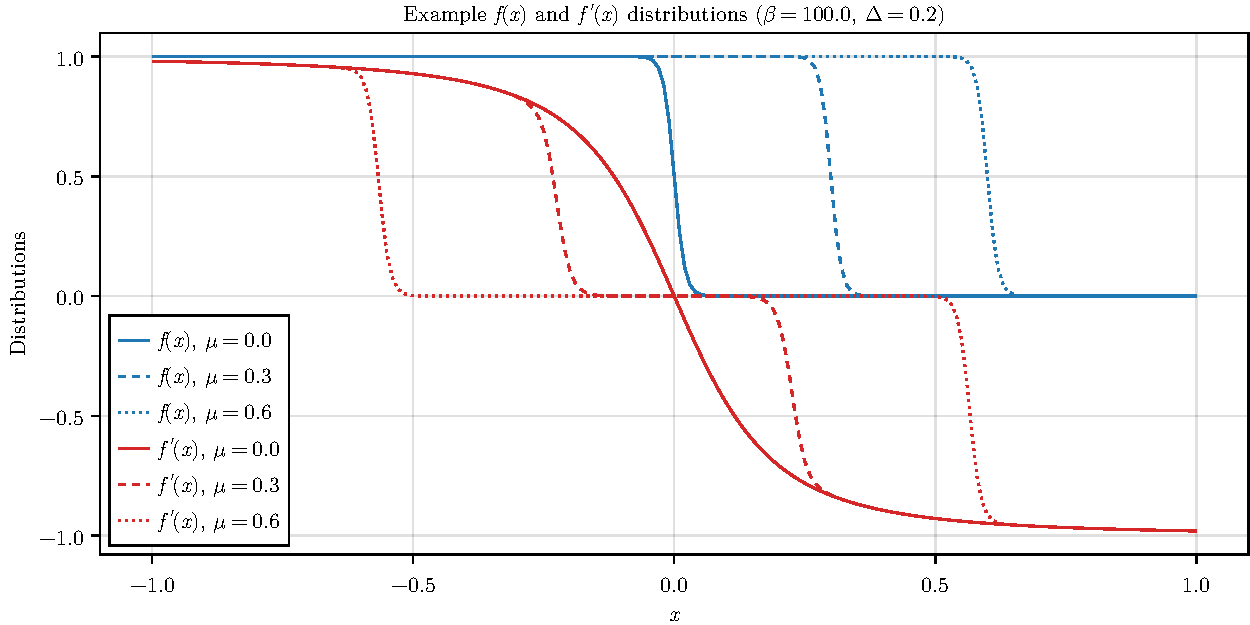
\includegraphics[width=0.9\linewidth]{../Project/src/labs/bin/pseudo-dirac.pdf}
	\caption{Sketch of the Fermi-Dirac distribution $f(x)$ and the pseudo-distribution $f'(x)$ described in text for the normal phase. These example data have been plotted arbitrarily at $mU=\Delta=0.2$ for $\mu=0.0,0.3,0.6$.}
	\label{fig:pseudo-dirac}
\end{figure}
%
These points end the proof: as anticipated, $f'$ is a monotonically descendent function of $\epsilon_\mathbf{k}$, a feature that allows us to re-use the entire derivation of Sec.~\ref{subsec:normal-bands-shrinking-C2} without hesitation, and conclude that also for the AF phase
\[
	u^{(d)} = 0
\]
while $u^{(s^*)}$ remains constrained in the limits of Eq.~\eqref{eq:af-us*-constraint}. Starting from a rather complicated scenario, we were able to resolve all the AF HFPs down to the pair
\[
	m, u^{(s^*)}
\]
Perhaps not-so-excitingly, the real net effect of the non-local extension of the HM is, once again, the shrinking effect on bands. Now it is a matter of numeric analysis to assess if Mott localization takes place.

\section{Discussion of numeric results}\label{sec:af-numeric}

In this section we present numeric results. For the AF phase, the HFPs vector, as we thoroughly showed, has two components
\[
	\mathbf{v} = \begin{bmatrix}
		m \\ u^{(s^*)}
	\end{bmatrix}
	\qquad
	\mathbf{v} = \mathbb{R}^2
\]
The resulting model RMPs are, as before:
\[
\begin{aligned}
	\tilde{t}_{ij} &\equiv \left(
	t - \frac{u^{(s^*)}V}{2}
	\right) \varphi_{ij}^{(s^*)} \\
	\tilde{\mu} &\equiv \mu + n (2zV-U)
\end{aligned}
\]
In the end, the computational scenario is not so different from the normal phase. The only real difference is our choice of parametric boundaries for simulations:
\[
	U = 0,~0.5,~1.0,~\dots,~20.0
	\qquad
	V = 0,~0.1,~0.2,~\dots,~4.0
	\qquad
	\delta = 0.0
\]
while we set $\delta=0.0$. {\color{tabred}As we anticipated in Sec.~\ref{subsec:af-instability}, any finite doping implies immediate disruption of commensurate antiferromagnetism, a consideration that makes any simulation at $\delta >0$ os low physical significance.}

\todo

\begin{figure}
	\centering
	\subfloat[Heatmap of $m$ in $UV$ plane.]{
		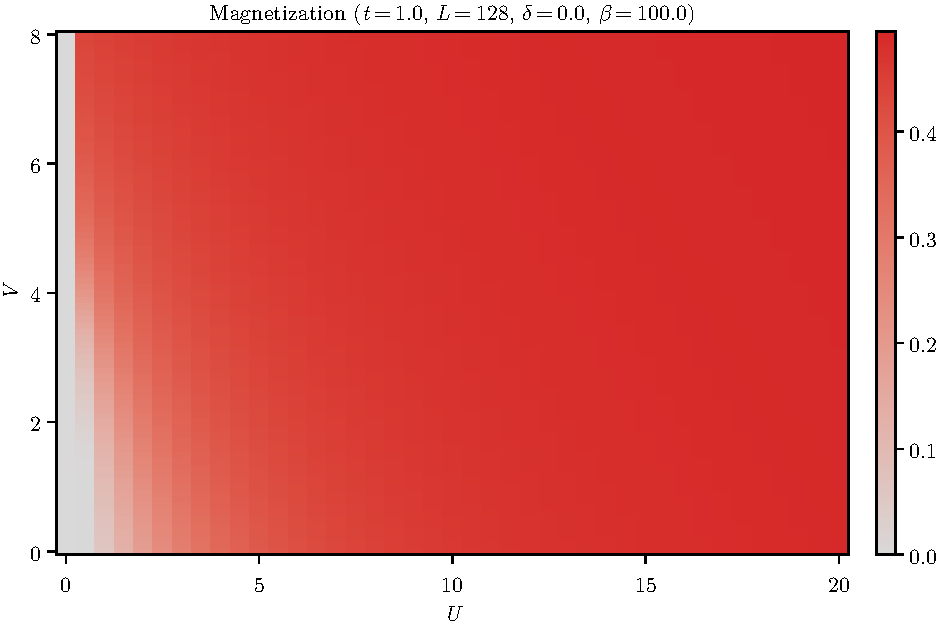
\includegraphics[height=0.32\linewidth]{../Project/plots/refined/Mode=rs/Phase=AF/Setup=A[128]/Syms=/RB=S/Obj=HFPs/xVar=U_yVar=V/m_t=1.0_L=128_δ=0.0_β=100.0.pdf}
		\label{subfig:af-m-data-A128}
	}
	\subfloat[Heatmap of $u^{(s^*)}$ in $UV$ plane.]{
		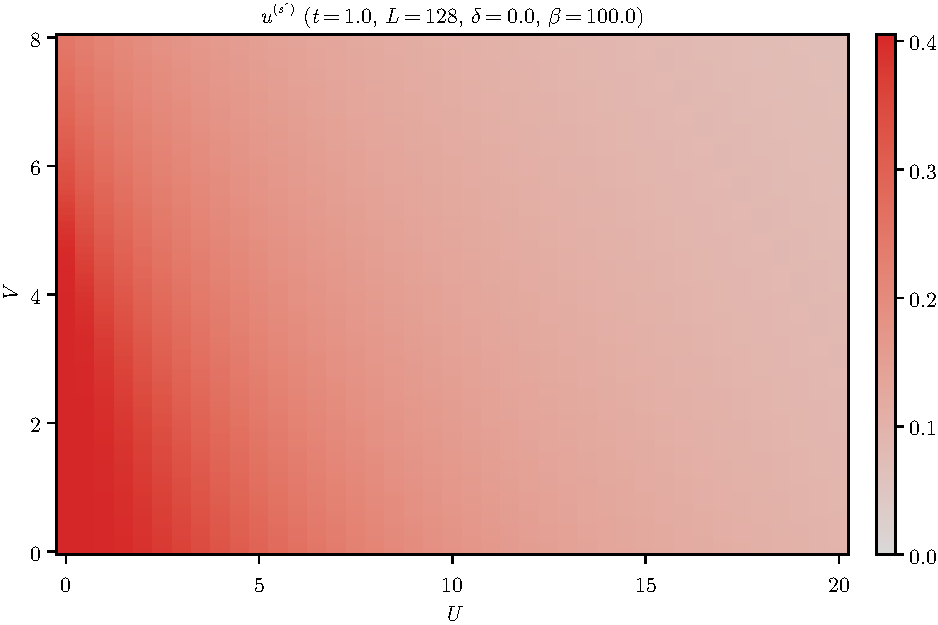
\includegraphics[height=0.32\linewidth]{../Project/plots/refined/Mode=rs/Phase=AF/Setup=A[128]/Syms=/RB=S/Obj=HFPs/xVar=U_yVar=V/uS_t=1.0_L=128_δ=0.0_β=100.0.pdf}
		\label{subfig:af-uS-data-A128}
	}	
	\caption{Plot of the self-consistent convergence values for the HFPs $m$ and $u^{(s^*)}$ in the AF phase.}
	\label{fig:af-data-A128}
\end{figure}


\begin{figure}
	\centering
	\subfloat[$U$-dependency of $m$ varying $V$.]{
		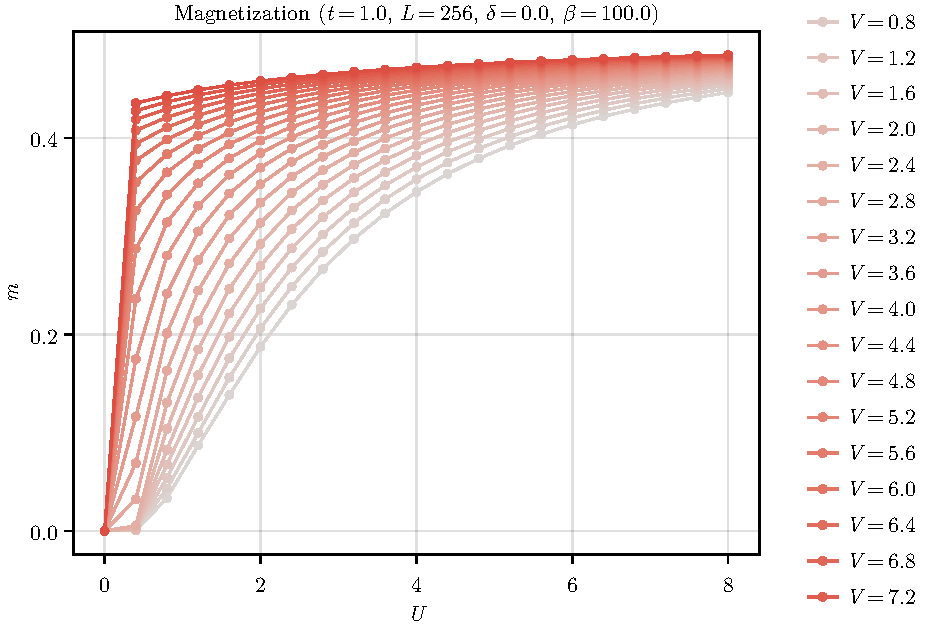
\includegraphics[height=0.32\linewidth]{../Project/plots/refined/Mode=hs/Phase=AF/Setup=A[256]/Syms=/RB=S/Obj=HFPs/xVar=U_pVar=V/m_t=1.0_L=256_δ=0.0_β=100.0.pdf}
		\label{subfig:af-m-data-A256-pVar=V}
	}
	\subfloat[$V$-dependency of $m$ varying $U$.]{
		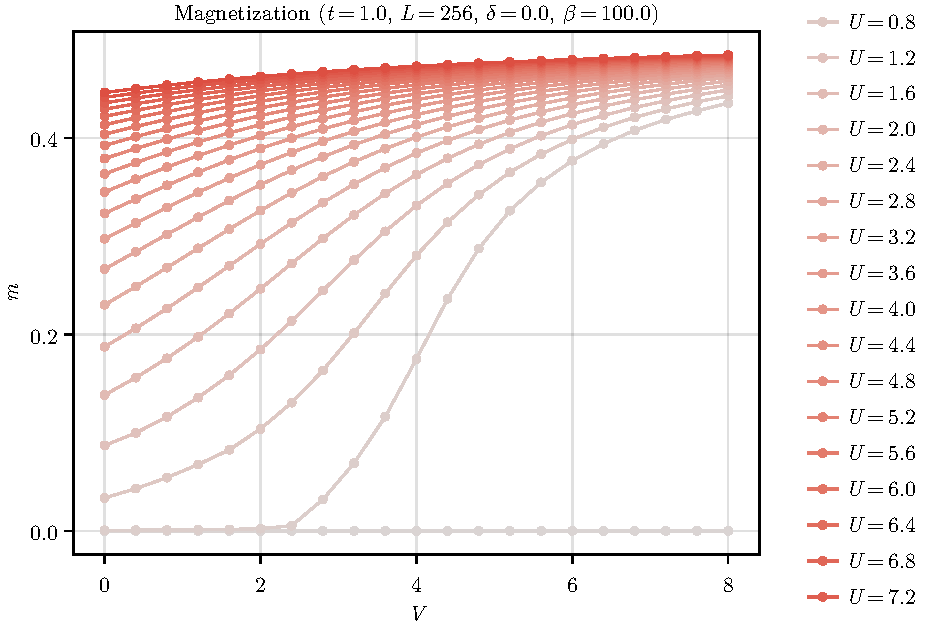
\includegraphics[height=0.32\linewidth]{../Project/plots/refined/Mode=hs/Phase=AF/Setup=A[256]/Syms=/RB=S/Obj=HFPs/xVar=V_pVar=U/m_t=1.0_L=256_δ=0.0_β=100.0.pdf}
		\label{subfig:af-m-data-A256-pVar=U}
	}\\[0.5em]
	\subfloat[$U$-dependency of $u^{(s^*)}$ varying $V$.]{
		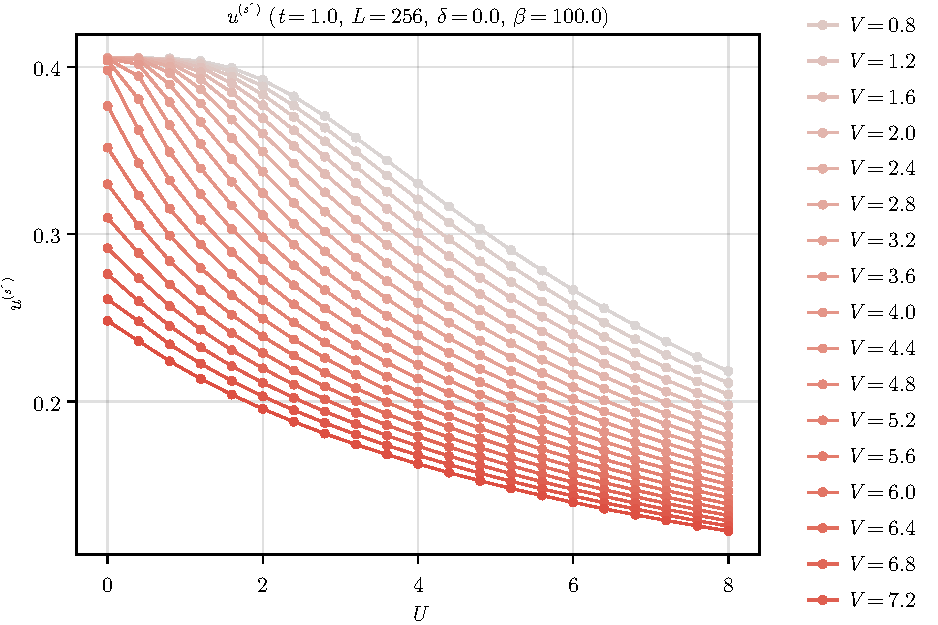
\includegraphics[height=0.32\linewidth]{../Project/plots/refined/Mode=hs/Phase=AF/Setup=A[256]/Syms=/RB=S/Obj=HFPs/xVar=U_pVar=V/uS_t=1.0_L=256_δ=0.0_β=100.0.pdf}
		\label{subfig:af-uS-data-A256-pVar=V}
	}
	\subfloat[$V$-dependency of $u^{(s^*)}$ varying $U$.]{
		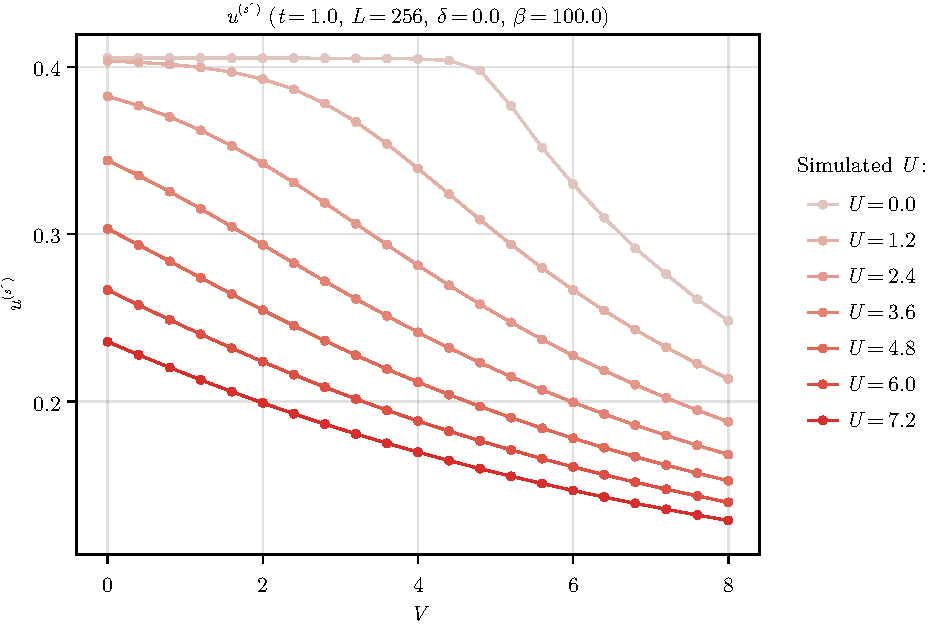
\includegraphics[height=0.32\linewidth]{../Project/plots/refined/Mode=hs/Phase=AF/Setup=A[256]/Syms=/RB=S/Obj=HFPs/xVar=V_pVar=U/uS_t=1.0_L=256_δ=0.0_β=100.0.pdf}
		\label{subfig:af-uS-data-A256-pVar=U}
	}
	\caption{Plot of the self-consistent convergence values for the HFPs $m$ and $u^{(s^*)}$ in the AF phase.}
	\label{fig:af-data-A256}
\end{figure}